%%%%%%%%%%%%%%%%%%%%%%%%%%%%%%%%%%%%%%%%%%%%%%%%%%%%%%%%%%%%%%%%
\chapter{Le traitement des données FIRSTv2}
\label{sec:DataReduction}
\setcounter{figure}{0}
\setcounter{table}{0}
\setcounter{equation}{0}

\minitoc

\clearpage
L'objectif de cette section est de présenter les données de \ac{FIRSTv2}, depuis leur acquisition et les procédures mises en place dans ce cadre jusqu'à leur traitement. Il s'agit aussi de présenter le formalisme mathématique de ce traitement de données afin d'établir les observables que l'on infère des données de \ac{FIRSTv2}.

% On the sensitivity of closure phases to faint companions in optical long baseline interferometry https://ui.adsabs.harvard.edu/abs/2012A%26A...541A..89L/abstract

%%%%%%%%%%%%%%%%%%%%%%%%%%%%%%%%
\section{L'acquisition des données}

%%%%%%%%%%%%%%%%
\subsection{Morphologie des images}

%%%%%%%%
\subsubsection{Étalonnage du détecteur}
\label{sec:CameraDark}

Comme décrit dans la section~\ref{sec:InstruCamera}, les images sont d'une taille de $2\,160 \,$px de hauteur par $2\,559 \,$px de largeur. La figure~\ref{fig:DarkFull} montre, à gauche, une image sans frange prise avec un temps d'exposition de $100 \,$ms et à droite la médiane d'un cube de $100$ images sans frange au même temps d'exposition. Ces images permettent de caractériser le courant d'obscurité et le bruit du détecteur de la caméra. 

Un tel cube sans frange est systématiquement acquis à chaque prise de données interférométriques. Le début du traitement des images consiste au calcul de la médiane de ce cube sans frange qui est ensuite soustraite aux images interférométriques diminuant ainsi le biais du détecteur et les structures fixes mentionnées dans le paragraphe précédent, présents sur toutes les données. Afin d'effectuer cette soustraction sans se soucier d'une possible dépendance non linéaire du courant d'obscurité du détecteur en fonction du temps d'exposition, ce dernier est choisi identique pour les deux types de données (sans et avec franges).

\begin{figure}[ht!]
    \begin{subfigure}{.5\textwidth}
        \centering
        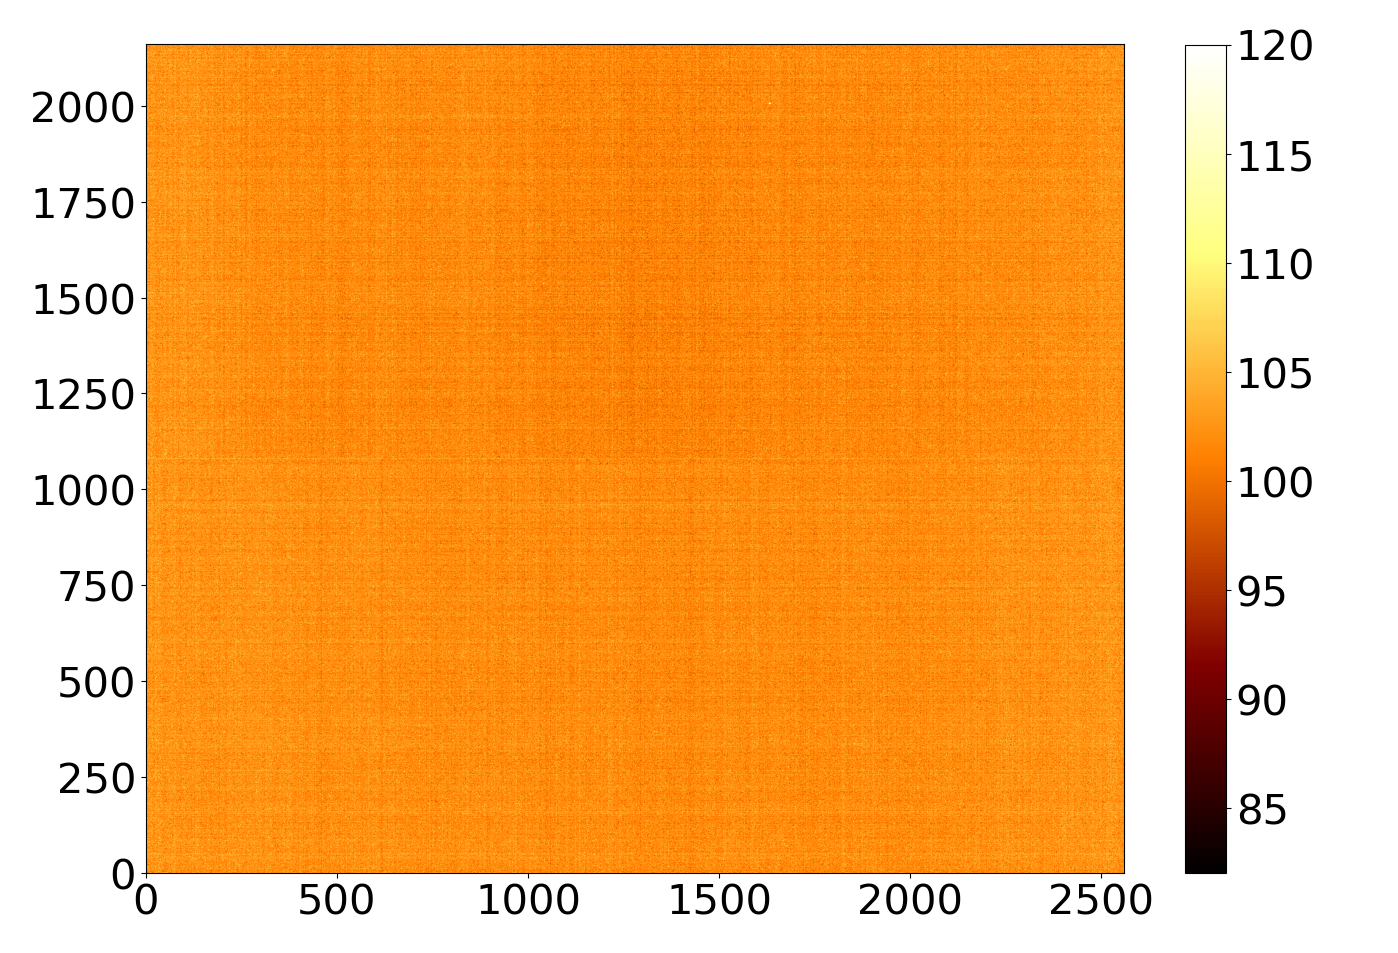
\includegraphics[width=\textwidth]{Figure_Chap3/20220705_DarkFullImage_100ms_24C_Im0_clip.png}
    \end{subfigure}%
    \begin{subfigure}{.5\textwidth}
        \centering
        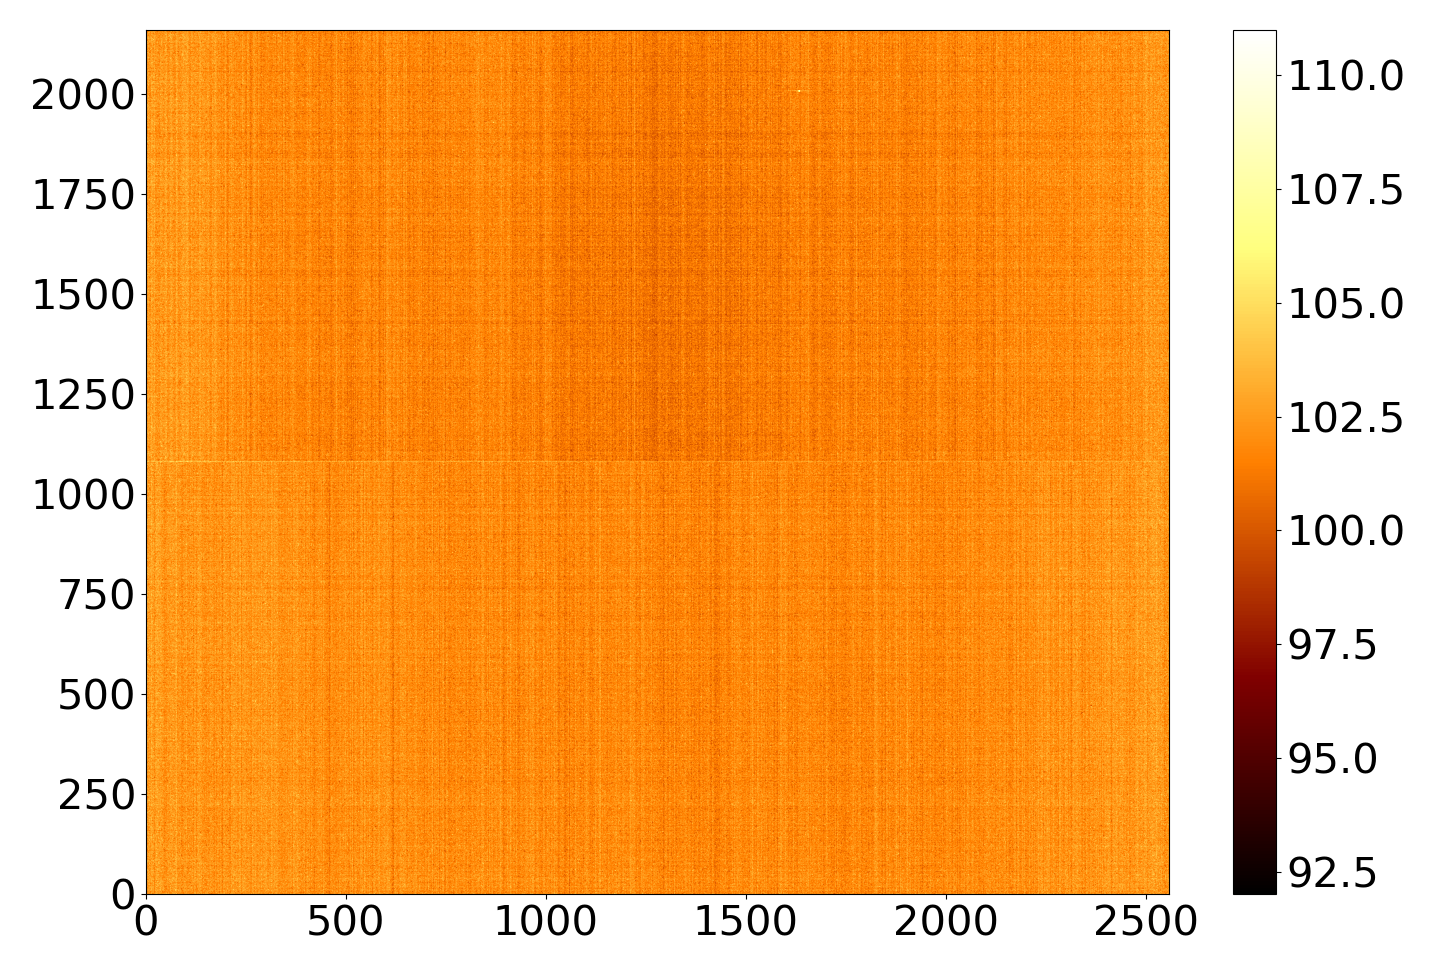
\includegraphics[width=\textwidth]{Figure_Chap3/20220705_DarkFullImage_100ms_24C_median_clip.png}
    \end{subfigure}
    \caption[Images du courant d'obscurité de la caméra de FIRSTv2.]{A gauche une image de la caméra non illuminée et à droite la médiane de $100$ de ces images, pour le même temps d'exposition de $100 \,$ms. Les valeurs des pixels données sur les échelles sont en \ac{ADU}.}
    \label{fig:DarkFull}
\end{figure}


%%%%%%%%
\subsubsection{Les images interférométriques}

Les images acquises avec la caméra sont rognées pour cadrer les sorties de la puce d'optique intégrée. La puce $Y$ a $10$ sorties et la puce $X$ a $20$ sorties, qui peuvent être dédoublées lorsqu'elles sont imagées par la caméra quand le prisme de wollaston est installé sur le chemin optique. Les différentes configurations possibles peuvent donc amener à avoir $10$, $20$ ou $40$ sorties à cadrer. Ce rognage dépend aussi de la bande spectrale de la source utilisée (changeant la largeur de l'image) et est choisi de façon à encadrer celle-ci le plus largement possible. Pour chaque montage sur le banc toutes les images (sans franges, \textit{flats} ou interférométriques) sont acquises avec le même rognage. La figure~\ref{fig:FringeCrop} présente deux images obtenues avec la caméra avec les sorties de la puce $X$ imagées sans que le prisme de wollaston soit installé ($20$ sorties sont donc visibles). La \sk est la source utilisée et les images ont alors une taille de $320 \,$px par $1\,800 \,$px ($1\,800$ canaux spectraux). En haut est montrée la médiane de $300$ images sans frange, qui est soustraite à une image avec des franges dont le résultat est montré en bas, pour un temps d'exposition de $50 \,$ms.

\begin{figure}[ht!]
    \centering
    \begin{subfigure}{\textwidth}
        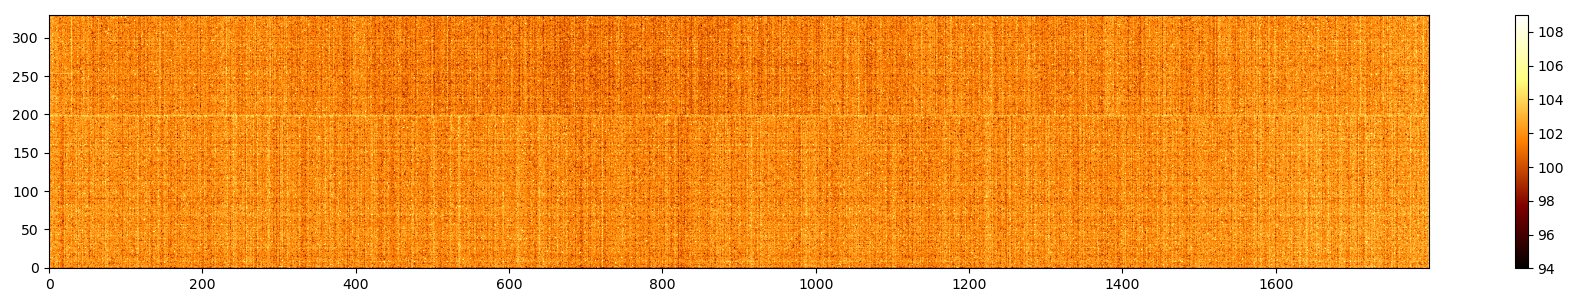
\includegraphics[width=\textwidth]{Figure_Chap3/20220614_P2VM_Dark1_50ms_median300.png}
    \end{subfigure}
    \begin{subfigure}{\textwidth}
        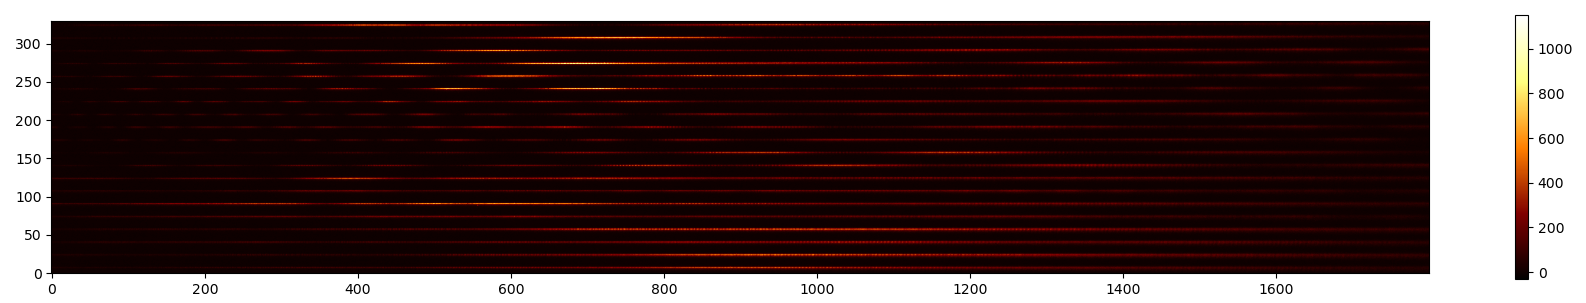
\includegraphics[width=\textwidth]{Figure_Chap3/20220614_P2VM_FullOn_001_50ms_Im0_SubDark.png}
    \end{subfigure}
    \caption[Image interférométrique obtenues sur FIRSTv2.]{En haut la médiane de $300$ images de la caméra sans franges et en bas une image avec des franges, avec la source \sk. Les deux images ont été acquises avec un temps d'exposition de $50 \,$ms et le même rognage induisant une taille d'image de $320 \, px$ de hauteur par $1\,800 \, px$ de largeur.}
    \label{fig:FringeCrop}
\end{figure}

Les lignes à retard sont au voisinage de leur position d'\ac{OPD} nulle, ce qui se traduit par la présence de franges sur l'image du bas. Il y a donc pour chacun des $1\,800$ canaux spectraux, un point de mesure du flux interférométrique pour chaque sortie, correspondant à une valeur d'\ac{OPD}. L'objectif est alors de reconstruire toutes les figures d'interférences par la mesure du flux des sorties pour au moins $4$ valeurs d'\ac{OPD}s par base. A cette fin, nous avons besoin de contrôler en piston les cinq segments du \ac{MEMS} qui illuminent les cinq entrées de la puce selon la méthode décrite dans la section~\ref{sec:Modulation}.


%%%%%%%%%%%%%%%%
\subsection{Étalonnage spectral}
\label{sec:EtalonnageSpectral}

Ici on souhaite associer à chaque pixel une valeur de longueur d'onde. Pour cela, j'utilise une lampe à vapeur de néon (Avalight-CAL-NEON par Avantes, avec sortie fibrée FC-PC). Le spectre d'émission de la vapeur de Néon est connu et présente de nombreuses raies sur la bande spectrale détectée par \ac{FIRSTv2}. La figure~\ref{fig:NeonReference} montre deux spectres de référence de l'émission de la vapeur de Néon, que j'ai utilisés pour les étalonnages spectraux durant ma thèse, celui de gauche étant un spectre que j'ai trouvé sur le site internet Astrosurf\footnote{\url{http://www.astrosurf.com/buil/us/spe2/calib2/neon1.gif}} et le deuxième étant celui mesuré par \ac{FIRSTv1} pendant la thèse d'Elsa Huby. Les deux spectres présentent des pics d'émission à des longueurs d'onde différentes et permettent donc d'identifier toutes les raies mesurées par \ac{FIRSTv2}.

\begin{figure}[ht!]
    \centering
    \begin{subfigure}{0.9\textwidth}
        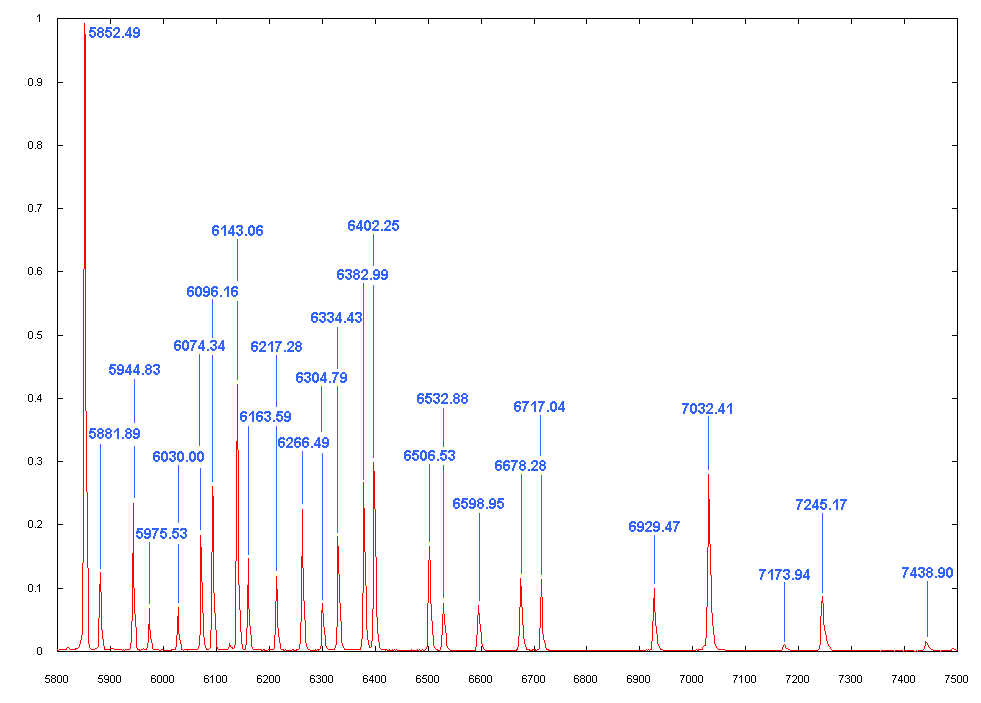
\includegraphics[width=\textwidth]{Figure_Chap3/Neon_SpectrumReference_Astrosurf.png}
    \end{subfigure}
    \begin{subfigure}{0.9\textwidth}
        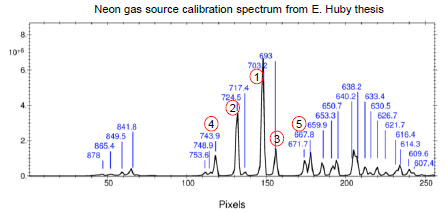
\includegraphics[width=\textwidth]{Figure_Chap3/Neon_SpectrumReference_ThesisEHuby.png}
    \end{subfigure}
    \caption[Spectres de référence d'émission du Néon utilisés pour l'étalonnage spectral de FIRSTv2.]{Spectres de références d'émission du Néon utilisés pour l'étalonnage spectral de FIRSTv2. À gauche est un spectre trouvé sur le site Astrosurf, présentant l'intensité des raies d'émissions du Néon (axe des ordonnées) en fonction de la longueur d'onde en Angstrom (axe des abscisses). À droite est le spectre tel que mesuré par FIRSTv1 pendant la thèse d'Elsa Huby traçant l'intensité des raies d'émission du Néon (axe des ordonnées) en fonction des pixels (axe des abscisses) de la caméra utilisée. Sur les deux spectres la longueur d'onde des pics est notée sur le graphique au-dessus de chaque pic.}
    \label{fig:NeonReference}
\end{figure}

La méthodologie utilisée pour conduire l'étalonnage spectral est la suivante :

\begin{enumerate}
    \item cinq séquences d'images sont acquises en illuminant successivement les cinq entrées de la puce avec la lampe néon;
    \item la somme des cinq moyennes de ces séquences est calculée pour donner une unique image avec toutes les sorties de la puce;
    \item une première étape d'identification des raies est effectuée avec une fonction de détection de pics pour chaque sortie;
    \item ensuite ces positions des pics sont passées en paramètres d'une fonction d'ajustement gaussien, afin de calculer finement la position centrale des pics et permettre leur identification en longueur d'onde;
    \item enfin, les longueurs d'ondes des pics sont ajustées aux positions des pics à l'aide d'une fonction polynomiale de degré 4.
\end{enumerate}

La figure~\ref{fig:NeonSpecCal} du haut montre l'image résultante de l'étape \textit{1.} en échelle logarithmique, la courbe du milieu montre l'identification précise des pics à l'issue de l'étape \textit{4.} sur le spectre d'émission de la lampe néon mesurée sur la sortie 1 de \ac{FIRSTv2} et la courbe du bas présente l'ajustement polynomial de l'étape \textit{5.}, pour la sortie 1 également. L'équation du polynôme trouvée par ajustement est montrée dans la légende et on remarque que la répartition des longueurs d'ondes sur les pixels du détecteur suit une loi affine. Cet ajustement a l'avantage de permettre l'extrapolation du modèle sur l'entièreté du détecteur, ce qui est utile lorsqu'on utilise la source \sk qui a une plus large bande que la lampe néon. Finalement, nous disposons d'autant d'équations de cet ajustement qu'il y a de sorties imagées sur la caméra et elles seront utilisées dans la suite du traitement de données, à chaque calcul en fonction de la longueur d'onde (notamment sur les phases) ou à chaque fois que des courbes seront tracées en fonction de la longueur d'onde. Enfin, il est indiqué dans le titre du graphique du milieu la résolution spectrale mesurée lors de l'étalonnage, qui est ici de $3\,184$ à $651 \,$nm. Elle a été mesurée sur toutes les sorties en moyenne à $3\,254$ avec un écart-type de $127$.

\begin{figure}[ht!]
    \centering
    \begin{subfigure}{0.8\textwidth}
        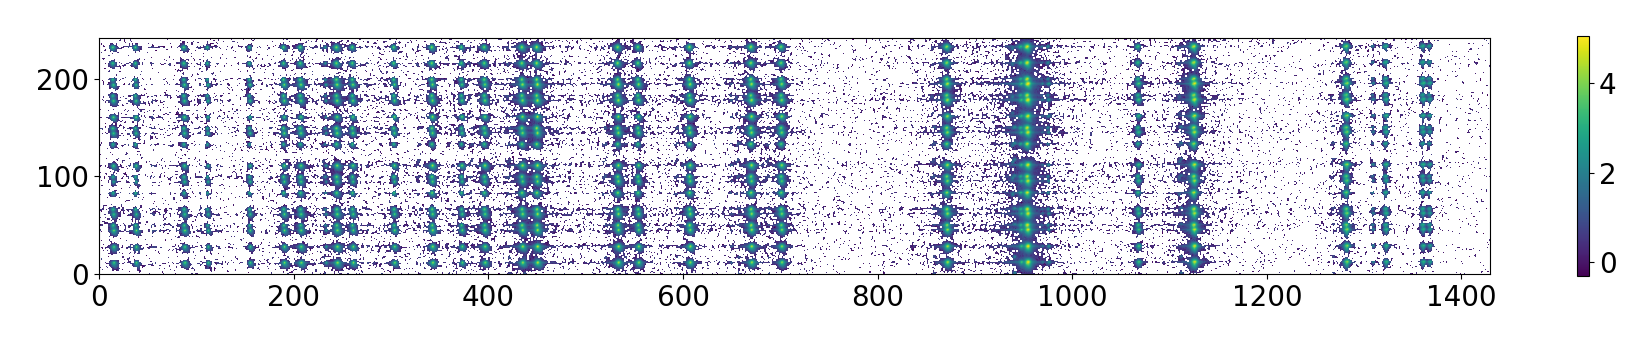
\includegraphics[width=\textwidth]{Figure_Chap3/20210722_5TC_Y_5InputsSum_Neon.png}
    \end{subfigure}
    \begin{subfigure}{0.8\textwidth}
        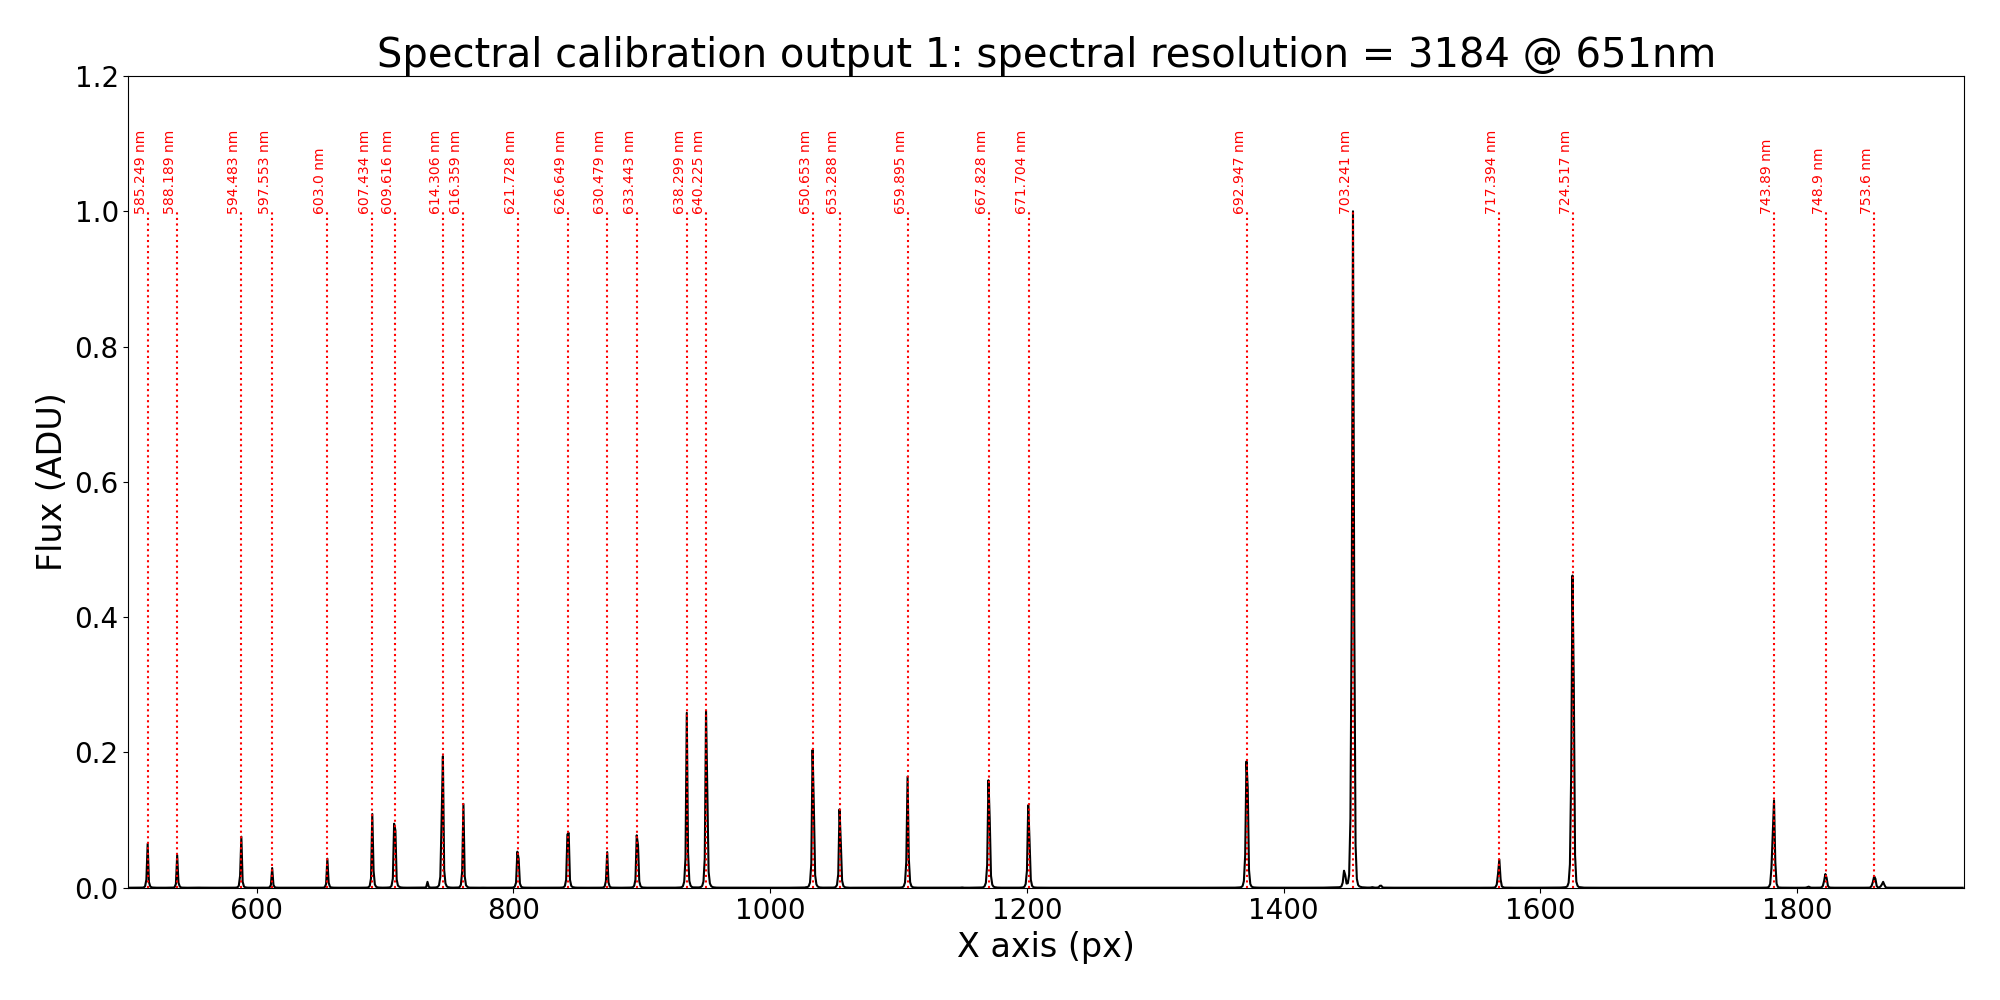
\includegraphics[width=\textwidth]{Figure_Chap3/20210722_5TC_PY_SpectralCalFlux01_Neon.png}
    \end{subfigure}
    \begin{subfigure}{0.8\textwidth}
        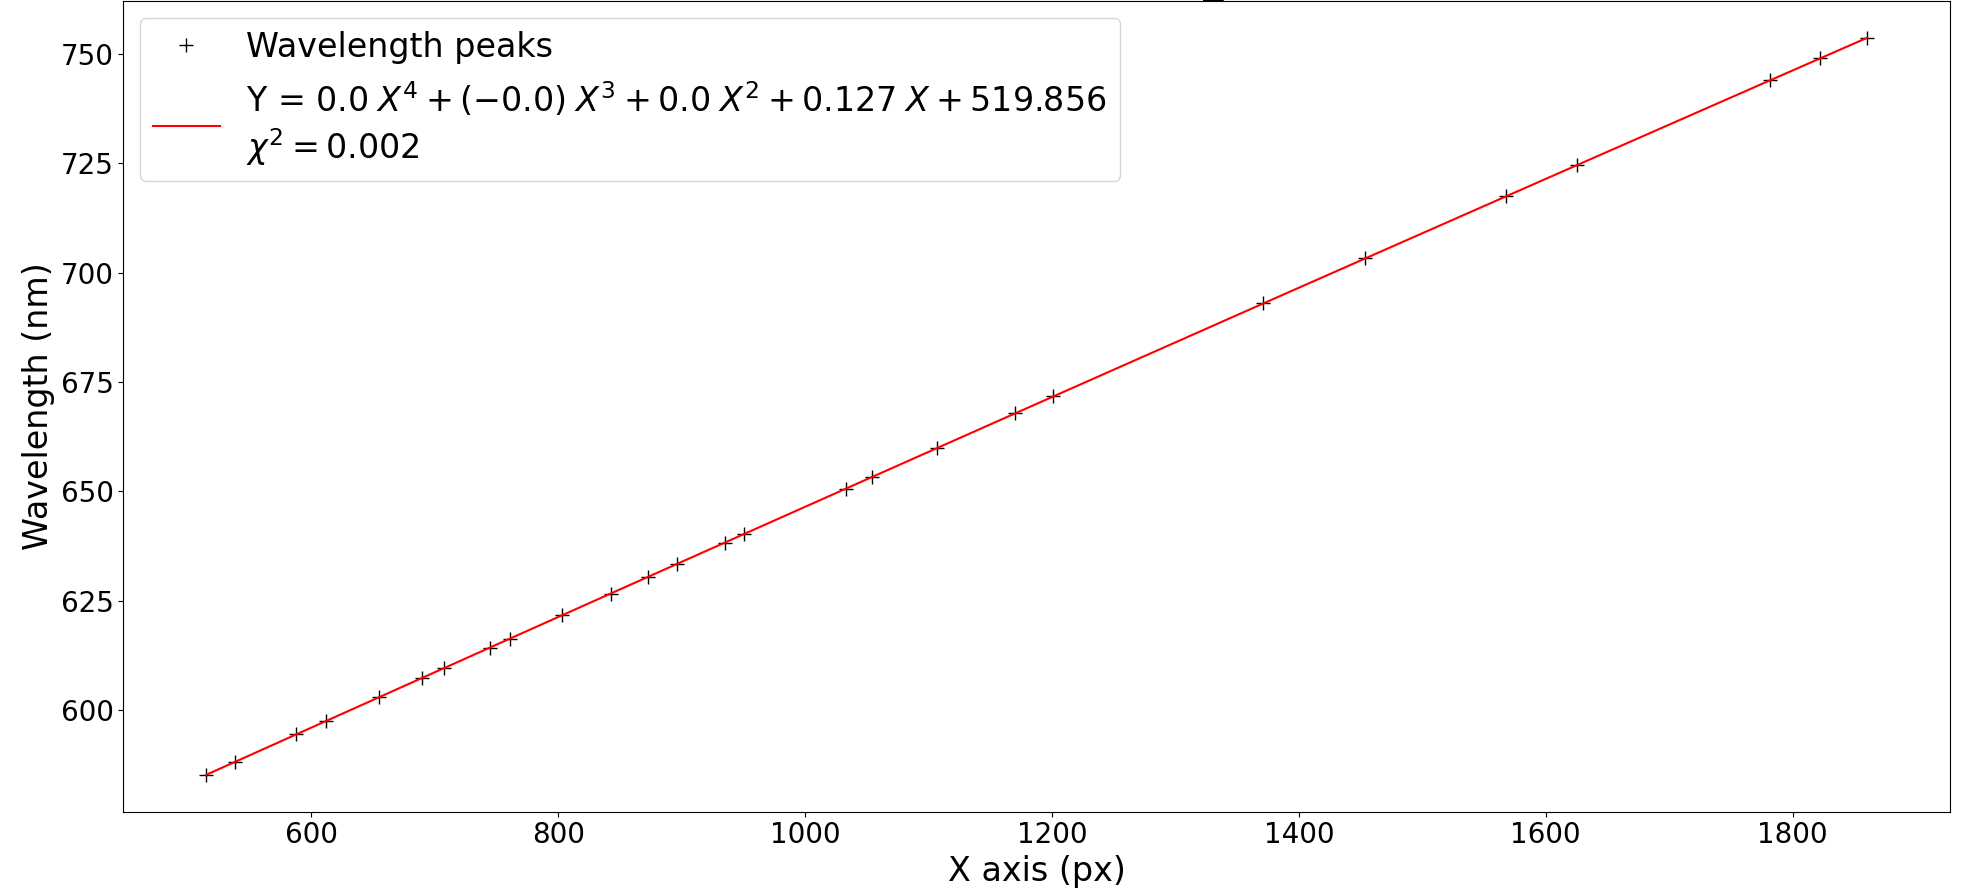
\includegraphics[width=\textwidth]{Figure_Chap3/20210722_5TC_Y_SpectralCalFitFort01_Neon_Manuscript.png}
    \end{subfigure}
    \caption[Résultat de l'étalonnage spectrale de FIRSTv2 avec une lampe spectrale au néon.]{Étalonnage spectral de FIRSTv2 à l'aide d'une lampe spectrale au néon. En haut : image de la caméra avec le spectre de la lampe néon sur chaque sortie. Au milieu : identification des pics du spectre du néon sur les pixels de la caméra pour la sortie 1. En bas : les longueurs d'onde du néon en fonction des positions des pics sur la caméra ainsi que l'ajustement polynomial associé, de la sortie 1.}
    \label{fig:NeonSpecCal}
\end{figure}


%%%%%%%%%%%%%%%%
\subsection{La modulation des franges}
\label{sec:Modulation}

L'acquisition des données interférométriques s'effectue en modulant les franges à l'aide des \ac{MEMS}. Ces derniers sont synchronisés avec la caméra de telle sorte que chaque image d'une séquence contienne les franges pour une valeur différente d'\ac{OPD}. La figure~\ref{fig:FringeSamplingABCD} montre la méthode ABCD utilisée pour mesurer une frange, représentée sur le graphique par une période de la fonction sinusoïdale ($2 \pi$). Cette période est divisée en $8$ et un déphasage de $\frac{3}{8} 2 \pi \,$rad, $\frac{-1}{8} 2 \pi \,$rad, $\frac{1}{8} 2 \pi \,$rad et $\frac{-3}{8} 2 \pi \,$rad est appliqué sur chaque base pour mesurer quatre points de la frange. Pour cela on applique quatre valeurs de piston sur deux segments du \ac{MEMS}, définis comme multiples de la longueur d'onde, prise égale à $750 \,$nm : $\frac{3}{8} \frac{0.750}{4} \,$\um, $\frac{-1}{8} \frac{0.750}{4} \,$\um, $\frac{1}{8} \frac{0.750}{4} \,$\um~et $\frac{-3}{8} \frac{0.750}{4} \,$\um. Comme ce sont les valeurs mises en consignes des segments, deux facteurs $1/2$ sont présents pour prendre en compte que (1) l'\ac{OPD} effective est la somme des déplacements de $2$ segments ainsi que (2) la lumière parcourt deux fois la même distance en étant réfléchie sur les segments.

\begin{figure}[htp!]
    \centering
    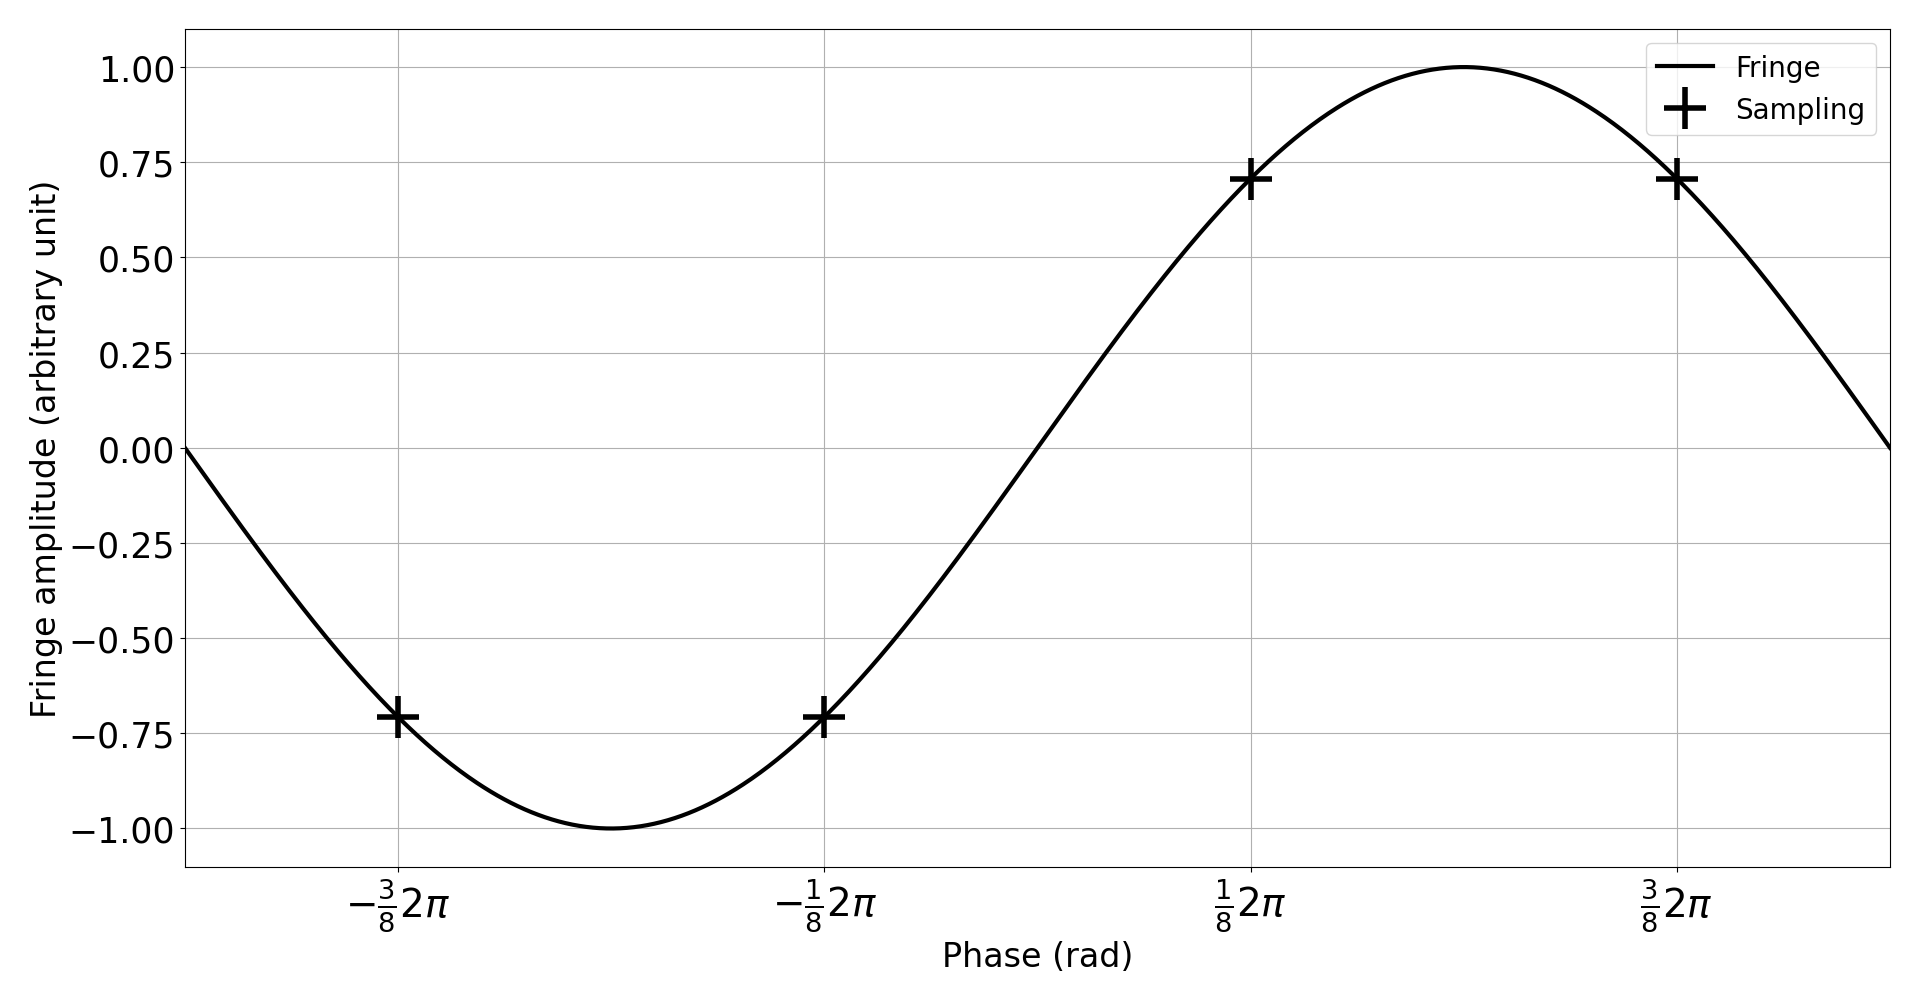
\includegraphics[width=\figwidth]{Figure_Chap3/Fringe_Sampling_ABCD.png}
    \caption[Méthode ABCD d'échantillonnage d'une frange.]{Méthode ABCD d'échantillonnage d'une frange. Ici la frange est représentée par une période de la fonction sinusoïdale ($2 \pi$) et pour l'échantillonner, les quatre valeurs de déphasage égales à $\frac{3}{8} 2 \pi \,$rad, $\frac{-1}{8} 2 \pi \,$rad, $\frac{1}{8} 2 \pi \,$rad et $\frac{-3}{8} 2 \pi \,$rad sont appliquées par les segments du MEMS.}
    \label{fig:FringeSamplingABCD}
\end{figure}

Une première approche est d'appliquer quatre valeurs de pistons, successivement, par paire de segments, pour effectuer les quatre points de mesures par base, ce qui constitue une séquence de modulation de $20$ points de mesure. La figure~\ref{fig:ModSeq20} du haut montre les valeurs de piston (en couleur) appliquées aux segments (selon l'axe vertical) en fonction des étapes de modulation (selon l'axe horizontal). La figure du bas montre les valeurs effectives d'\ac{OPD}s tout au long de la séquence de modulation pour les dix bases. On remarque qu'il y a deux types de quadruplets de valeurs d'\ac{OPD}s dans cette séquence. Le premier type (aux valeurs les plus élevées sur la figure) contient les valeurs précédemment définies ($\frac{3}{8} \frac{0.750}{4} \,$\um, $\frac{-1}{8} \frac{0.750}{4} \,$\um, $\frac{1}{8} \frac{0.750}{4} \,$\um~et $\frac{-3}{8} \frac{0.750}{4} \,$\um) car elles sont obtenues en déplaçant deux segments et sont appliquées sur les bases $1-2$, $2-3$, $3-4$, $4-5$ et $1-5$. Le deuxième type contient quatre valeurs dont les amplitudes sont moitié moindres que celles du premier type ($\frac{3}{8} \frac{0.750}{8} \,$\um, $\frac{-1}{8} \frac{0.750}{8} \,$\um, $\frac{1}{8} \frac{0.750}{8} \,$\um~et $\frac{-3}{8} \frac{0.750}{8} \,$\um) car elles sont obtenues avec un des deux segments immobile et sont appliquées sur les bases $1-3$, $1-4$, $2-4$, $2-5$ et $3-5$. Par conséquent, la moitié des bases sont modulées sur une OPD deux fois trop petite ce qui ne permet pas un bon échantillonnage des franges et empêchant le code de traitement de données de converger.

\begin{figure}[ht!]
    \centering
    \begin{subfigure}{0.8\textwidth}
        \centering
        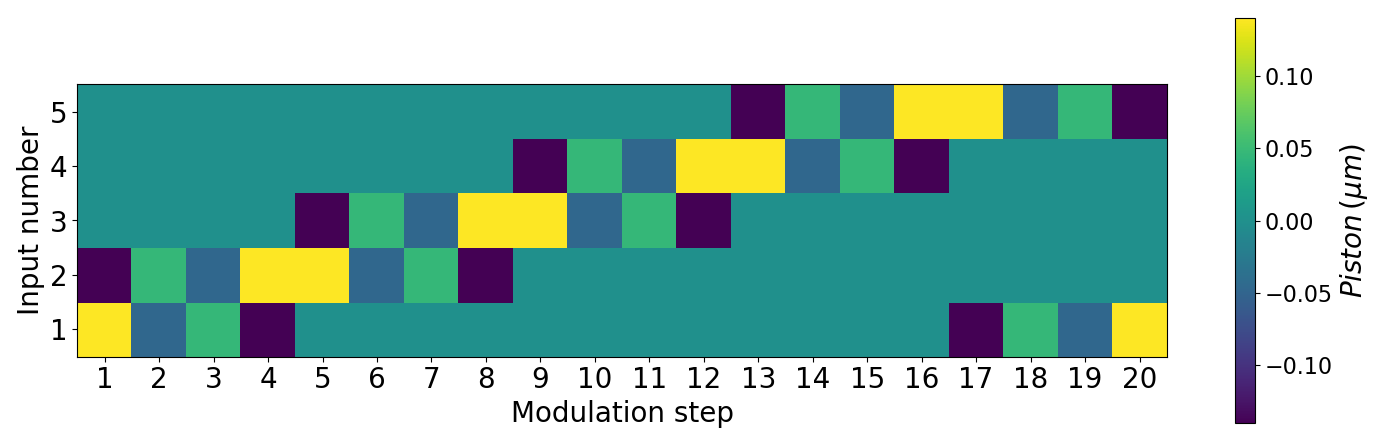
\includegraphics[width=\textwidth]{Figure_Chap3/20210503_MEMSModulationSequence_Standard_step20.png}
    \end{subfigure}
    \begin{subfigure}{0.8\textwidth}
        \centering
        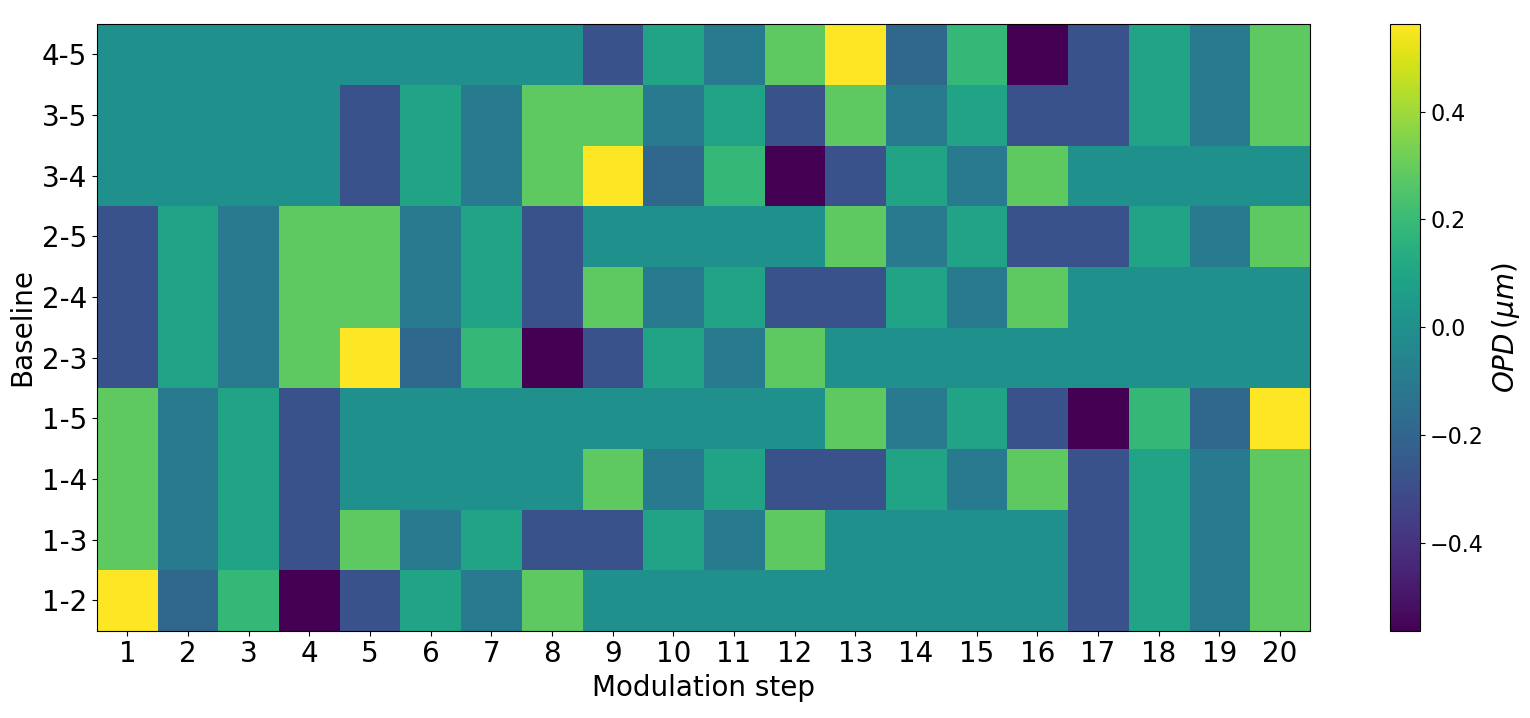
\includegraphics[width=\textwidth]{Figure_Chap3/20210503_MEMSModulationSequence_Standard_step20_DiffBase.png}
    \end{subfigure}
    \caption[Séquence basique de modulation des MEMS à 20 pas pour échantillonner les franges sur FIRSTv2.]{En haut la séquence des pistons (en $\upmu$m) appliqués aux cinq segments du MEMS qui illuminent les entrées de la puce. En bas les valeurs d'OPDs (en $\upmu$m) induites sur les dix bases en application de cette séquence de modulation. Les couleurs sont les valeurs appliquées, les axes horizontaux sont les étapes de la séquence et les axes verticaux sont les segments et les bases, respectivement, pour la figure du haut et du bas.}
    \label{fig:ModSeq20}
\end{figure}

Une deuxième approche est de moduler plusieurs bases en même temps et non une seule à la fois comme précédemment. Il faut alors s'assurer que chaque base soit modulée au moins une fois par le bon quadruplet de pistons durant la séquence de modulation. La figure~\ref{fig:ModSeq12} montre un exemple d'une telle séquence. De même que sur la figure~\ref{fig:ModSeq20}, en haut est présentée la séquence des pistons appliqués aux segments. Sur les quatre premiers pas, tous les segments sont modulés, la condition étant que la moitié des segments soient modulés avec des valeurs opposées à l'autre moitié (ici trois segments sont modulés de la même façon et deux sont modulés avec la valeur opposée). A partir de la figure du bas on peut voir les valeurs d'\ac{OPD}s induites sur les bases pour ces quatre premières étapes, nous permettant de définir les bases sur lesquelles appliquer le quadruplet pour les étapes suivantes. Ici seules les bases $1-3$, $1-5$, $2-4$ et $3-5$ ne sont pas modulées et doivent donc l'être par la suite. Ces quatre bases ne pouvant pas être modulées sur le bon quadruplet d'\ac{OPD}s en même temps, il faut alors les moduler sur huit étapes de plus. La séquence résultante est ainsi composée de $12$ étapes. Cette nouvelle séquence a les deux atouts suivants :

\begin{enumerate}
    \item elle permet la modulation des franges sur les quatre points d'échantillonnage, à la bonne amplitude;
    \item elle a aussi le bon goût d'être plus courte ($12$ étapes contre $20$) ce qui permet de réduire l'influence des perturbations atmosphériques (lorsque l'instrument fait des mesures sur ciel) et/ou présents sur le banc (mouvements d'air, vibrations, etc.).
\end{enumerate}

On note que la longueur de cette séquence peut être divisée par deux lorsqu'on utilise la puce $X$. En effet, avec cette puce, chaque image contient deux mesures de frange, théoriquement déphasées de $\pi \,$rad (voir la section~\ref{sec:ChipConcept}). Mais au cours de cette thèse, cette propriété de la puce $X$ n'a pas été utilisée et les interférogrammes mesurés avec cette puce ont été exploités séparément car il serait nécessaire d'écrire une partie en plus dans le programme de réduction de données et de faire de nouveaux tests pour vérifier la valeur du déphasage entre les couples de sorties. La même séquence de modulation a ainsi été utilisée pour les deux puces.

\begin{figure}[ht!]
    \centering
    \begin{subfigure}{0.8\textwidth}
        \centering
        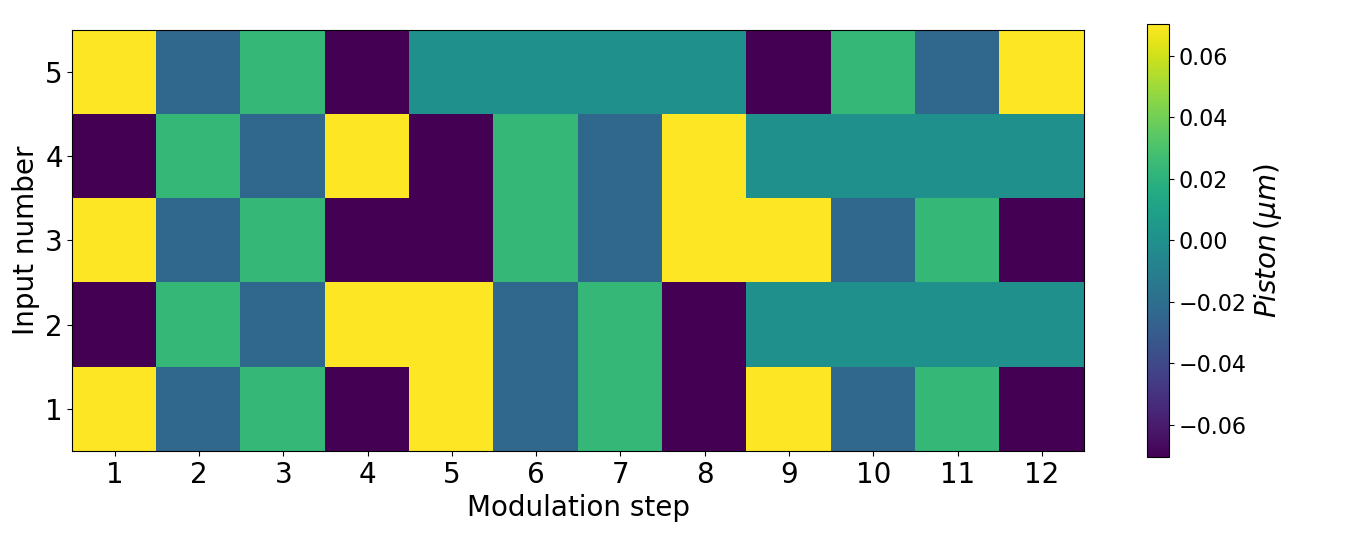
\includegraphics[width=\textwidth]{Figure_Chap3/20220826_MEMSModulationSequence_GoodSampling_step12.png}
    \end{subfigure}
    \begin{subfigure}{0.8\textwidth}
        \centering
        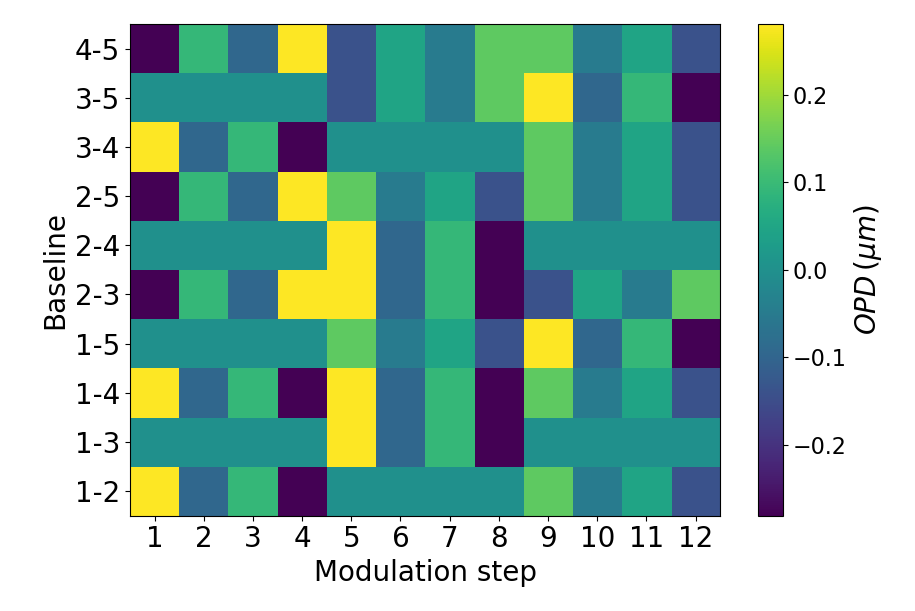
\includegraphics[width=\textwidth]{Figure_Chap3/20220826_MEMSModulationSequence_GoodSampling_step12_DiffBase.png}
    \end{subfigure}
    \caption[Séquence optimisée de modulation des MEMS à 12 pas pour échantillonner les franges sur FIRSTv2.]{En haut la séquence optimisée des pistons (en $\upmu$m) appliqués aux cinq segments du MEMS qui illuminent les entrées de la puce. En bas les valeurs d'OPDs (en $\upmu$m) induites sur les dix bases en application de cette séquence de modulation. Les couleurs sont les valeurs appliquées, les axes horizontaux sont les étapes de la séquence et les axes verticaux sont les segments et les bases, respectivement, pour la figure du haut et du bas.}
    \label{fig:ModSeq12}
\end{figure}


%%%%%%%%%%%%%%%%%%%%%%%%%%%%%%%%
\section{Étalonnage de l'instrument}

La méthode pour calculer les termes de visibilité complexe qui est utilisée dans le traitement des données de \ac{FIRSTv2} a été adaptée de celle déjà utilisée sur \ac{FIRSTv1} \citep{huby2012, huby2013these} et Vievard et al. (2023, en préparation).

%%%%%%%%%%%%%%%%
\subsection{L'interférométrie : une mesure de la cohérence des ondes lumineuses}

Pour écrire cette partie, je me suis beaucoup aidé du fabuleux cours de Guy Perrin, que j'ai pu suivre pendant ma deuxième année de master, sur l'interférométrie astronomique et qui fait référence dans le domaine.

Commençons par considérer une source astrophysique étendue incohérente à l'infini dans la direction $\vv{Z}$, émettant une onde lumineuse qui a pour champ électrique, au point $\vv{P}$ et à l'instant $t$ : $E(P,\vv{Z},t) = |E(P,\vv{Z},t)| e^{i(\omega t - \vv{k}.\vv{P})}$, avec le vecteur d'onde $\vv{k} = 2\pi \frac{\vv{Z}}{\lambda}$ et la pulsation $\omega = 2\pi \frac{c}{\lambda}$. Alors, en un point $P$ du foyer image d'un interféromètre qui combine deux faisceaux séparés par la base $\vv{B}$, est mesurée l'intensité $I_{tot}(\vv{B})$ de la superposition de deux champs électriques, intégré sur la surface de la source, selon l'équation :

\begin{align}
	I_{tot}(\vv{B}) &= \int_{source} \langle | E(P,\vv{Z},t) + E(P+\vv{B},\vv{Z},t) |^2 \rangle d^2\vv{Z} \label{eq:Interferogramme1} \\
	&= 2 \int_{source} I(\vv{Z},\lambda) d^2\vv{Z} + 2 \Re \left[\int_{source} I(\vv{Z},\lambda) e^{-2i\pi \vv{Z}.\frac{\vv{B}}{\lambda}} d^2\vv{Z} \right] \\
	&= 2 \int_{source} I(\vv{Z},\lambda) d^2\vv{Z} + 2 \left(\int_{source} I(\vv{Z},\lambda) d^2\vv{Z} \right) \Re [\mu_{nn'}(\vv{B})] \label{eq:Interferogramme3}
\end{align}

Où l'intensité lumineuse des deux faisceaux est supposée égale et où le facteur de cohérence complexe de la base $n-n'$ est défini selon :

\begin{equation}
    \mu_{nn'}(\vv{S}) = \frac{\int_{\alpha, \beta} I_{\lambda}(\alpha,\beta) e^{-2i\pi (\alpha u + \beta v)} d\alpha d\beta}{\int_{\alpha, \beta} I_{\lambda}(\alpha,\beta) d\alpha d\beta} \label{eq:ZVC}
\end{equation}

Avec $(\alpha,\beta)$ les coordonnées du vecteur $\vv{Z}$, $(u, v)$ les coordonnées du vecteur fréquence spatiale $\vv{S} = \vv{B}/\lambda$ projeté selon $\vv{Z}$. L'équation~\ref{eq:ZVC} est le résultat du théorème de Zernike - Van Cittert, qui énonce que la cohérence complexe est la transformée de Fourier de la distribution spatiale d'intensité de la source normalisée par le flux de cette dernière. C'est donc ce terme là que l'on cherche à mesurer pour obtenir des informations sur la cible observée. On l'appelle aussi communément la visibilité complexe que l'on note donc comme suit :

\begin{equation}
	\mu_{nn'} = |V_{nn'}| e^{i\varphi_{nn'}} A_n A_{n'} e^{i(\psi_{nn'} + \Delta\Phi_{nn'})} \label{eq:mu}
\end{equation}

Les termes $|V_{nn'}|$ et $\varphi_{nn'}$ sont, respectivement, le module et la phase de la visibilité complexe. $A_n$ et $A_{n'}$ sont, respectivement, le flux des sous-pupilles $n$ et $n'$. $\psi_{nn'}$ est le piston différentiel intrinsèque à l'instrument (résultant des \ac{OPD}s résiduelles entre les différentes fibres et autres aberrations optiques) dont nous verrons l'étalonnage dans la section~\ref{sec:P2VM}. Enfin, $\Delta\Phi_{nn'}$ est le piston atmosphérique correspondant aux aberrations non corrigées par l'optique adaptative (dans le cas où l'instrument est sur ciel) qui sera étalonné par la méthode d'analyse de données présentée dans la section~\ref{sec:PhaseSpecDiff}.

A partir d'une séquence d'images sur laquelle les franges sont modulées selon la séquence présentée dans la section~\ref{sec:Modulation}, l'interférogramme en fonction de l'\ac{OPD} est reconstruit et un modèle est ajusté pour en déduire les termes de visibilités complexes, comme décrit dans la section suivante.


%%%%%%%%%%%%%%%%
\subsection{Pixel-To-Visibility Matrix (la pitouvièm)}
\label{sec:P2VM}

Dans cette section, je vais exposer la partie du traitement de données consistant à retrouver les termes de visibilités complexes dans les interférogrammes mesurés. Il s'agit d'une méthode adaptée aux instruments possédant une pupille de sortie peu diluée (la dilution étant définie par le rapport entre les longueurs de base et le rayon des sous-pupilles), ce qui est le cas sur FIRSTv2. Elle a été pour la première fois utilisée pour les données de l'instrument \ac{AMBER} \citep{millour2004, tatulli2007} et consiste en la modélisation des franges dans le but de les ajuster et d'étalonner le terme complexe dû à l'instrument (le terme $e^{i(\psi_{nn'})}$ de l'équation~\ref{eq:mu}).

On commence par exprimer l'intensité de la base $n-n'$ de l'équation~\ref{eq:Interferogramme1}, avec un retard temporel $\updelta \text{t} = x / c$ (avec $x$ la variable spatiale discrète, selon l'axe des \ac{OPD}s) :

\begin{align}
    I_{nn'}(x) &= \int_{source} \langle | E(P,\vv{Z},t) + E(P+\vv{B},\vv{Z},t + \updelta \text{t}) |^2 \rangle d^2\vv{Z}
\end{align}

Et d'après l'équation~\ref{eq:Interferogramme3} combinée avec l'équation~\ref{eq:mu}, on écrit : 

\begin{align}
    I_{nn'}(x) &= \sum_{i \in \{n,n'\}} A_i^2 E_i^2 + 2 \Re \left[ A_n E_n A_{n'} E_{n'} e^{i(\frac{2 \pi}{\lambda}x + \varphi_{nn'} + \psi_{nn'} + \Delta\Phi_{nn'})}  \right] \\
    &= \sum_{i \in \{n,n'\}} A_{i}^{2} E_{i}^{2} + 2 A_n E_n A_{n'} E_{n'} cos \left(\frac{2 \pi}{\lambda}x + \varphi_{nn'} + \psi_{nn'} + \Delta\Phi_{nn'} \right)
\end{align}

Avec $A_i$ le flux et $E_i$ l'enveloppe de la cohérence temporelle, de la sous-pupille $i$. On considère les termes $A_i$ et $E_i$ indépendants de $x$. Les termes $A_i^2 E_i^2$ caractérisent notamment la transmission de la puce. En effet, chaque sortie imagée sur le détecteur est la combinaison interférométrique de faisceaux qui traversent des guides d'onde différents dans la puce.

En reformulant cette équation et en utilisant la relation~\ref{eq:mu}, on trouve une relation linéaire entre l'interférogramme $I_{nn'}(x)$ et le terme de cohérence complexe $\mu_{nn'}$, s'écrivant :

\begin{equation}
    I_{nn'}(x) = \sum_{i \in \{n,n'\}} A_{i}^{2} E_{i}^{2}(x) + \Re [\mu_{nn'}] C_{nn'}(x) + \Im [\mu_{nn'}] S_{nn'}(x) \label{eq:InterferogrammeLineaire}
\end{equation}

Avec
\begin{align}
    \left\{
    \begin{array}{r@{}l}\displaystyle
    &C_{nn'}(x) = 2E_n E_{n'}\cos \left( \frac{2 \pi}{\lambda}x \right) \\
    &S_{nn'}(x) = -2E_n E_{n'}\sin \left( \frac{2 \pi}{\lambda}x \right)
    \end{array}\right. \label{eq:V2PMtermesComplexes}
\end{align}

Ainsi, $\{ F_{nn'} \text{; } C_{nn'}(x) \text{; } S_{nn'}(x)  \}$ forme une base sur laquelle sont projetés les interférogrammes (avec $F_{nn'} = \sum_{i \in \{n,n'\}} A_{i}^{2} E_{i}^{2}$). Ce sont les termes qui contiennent les erreurs instrumentales de l'instrument et ils devront être étalonnés, comme cela sera montré plus loin.

Enfin, on peut ré-écrire l'équation~\ref{eq:InterferogrammeLineaire} pour toutes les bases sous forme matricielle, ce qui est plus adapté au calcul numérique. On note $n_B$ le nombre de bases correspondant à toutes les combinaisons par paire des faisceaux $n$ et $n'$ ($n_B = n_I(n_I-1)/2$ pour $n_I$ sous-pupilles), le nombre de pixels $n_p$ sur une séquence de modulation ($n_p = 12$ pour la séquence montrée dans la section~\ref{sec:Modulation}). La matrice est alors la concaténation en ligne des équations des interférogrammes de toutes les bases $b_i$. Pour $5$ sous-pupilles d'entrée, cette matrice s'écrit donc :

\begin{align}
    \text{\textbf{I}}=
    \begin{bmatrix}
    	I_{b_1}(x_1) \\
    	\vdots \\
    	I_{b_1}(x_{n_p}) \\
    	\vdots \\
    	I_{b_{n_B}}(x_1) \\
    	\vdots \\
    	I_{b_{n_B}}(x_{n_p})
    \end{bmatrix}
    = V2PM \cdot
    \begin{bmatrix}
        A_{1}^2 \\
        \vdots \\
        A_{n_I}^2 \\
        \Re [\mu_{b_1}] \\
        \vdots \\
        \Re [\mu_{b_{n_B}}] \\
        \Im [\mu_{b_1}] \\
        \vdots \\
        \Im [\mu_{b_{n_B}}]
    \end{bmatrix}
    =V2PM\cdot\text{\textbf{P}} \label{eq:IV2PMP}
\end{align}

% \begin{align}\tiny
%     \begin{bmatrix}
%         E_{1}^2(x_1)     & E_{2}^2(x_1)     &        & \vdots               & \vdots             & C_{b_1}(x_1)     &        & 0                    & S_{b_1}(x_1)     &        & 0 \\
%         \vdots           & \vdots           &        & \vdots               & \vdots             & \vdots           &        & \vdots               & \vdots           &        & \vdots \\
%         E_{1}^2(x_{n_p}) & E_{2}^2(x_{n_p}) &        & \vdots               & \vdots             & C_{b_1}(x_{n_p}) &        & 0                    & S_{b_1}(x_{n_p}) &        & 0 \\
%         \vdots           & \vdots           & \ddots & \vdots               & \vdots             & 0                & \ddots & 0                    & 0                & \ddots & 0 \\
%         \vdots           & \vdots           &        & E_{n_I-1}^2(x_1)     & E_{n_I}^2(x_1)     & 0                &        & C_{b_{n_B}}(x_1)     & 0                &        & S_{b_{n_B}}(x_1) \\
%         \vdots           & \vdots           &        & \vdots               & \vdots             & \vdots           &        & \vdots               & \vdots           &        & \vdots \\
%         \vdots           & \vdots           &        & E_{n_I-1}^2(x_{n_p}) & E_{n_I}^2(x_{n_p}) & 0                &        & C_{b_{n_B}}(x_{n_p}) & 0                &        & S_{b_{n_B}}(x_{n_p})
%     \end{bmatrix}
% \end{align}

avec V2PM =
\begin{align}\tiny
    \hspace{-1ex}\bordermatrix{
        & \tikzmark{harrowleft1} & & & & \tikzmark{harrowright1} & \tikzmark{harrowleft2} & & \tikzmark{harrowright2} & \tikzmark{harrowleft3} & & \tikzmark{harrowright3} \cr
        & E_{1}^2(x_1)     & E_{2}^2(x_1)     &        & \vdots               & \vdots             & C_{b_1}(x_1)     &        & 0                    & S_{b_1}(x_1)     &        & \hphantom{mmi} 0 \hphantom{mmii} \tikzmark{varrowtop} \cr
        & \vdots           & \vdots           &        & \vdots               & \vdots             & \vdots           &        & \vdots               & \vdots           &        & \vdots \cr
        & E_{1}^2(x_{n_p}) & E_{2}^2(x_{n_p}) &        & \vdots               & \vdots             & C_{b_1}(x_{n_p}) &        & 0                    & S_{b_1}(x_{n_p}) &        & 0 \cr
        & \vdots           & \vdots           & \ddots & \vdots               & \vdots             & 0                & \ddots & 0                    & 0                & \ddots & 0 \cr
        & \vdots           & \vdots           &        & E_{n_I-1}^2(x_1)     & E_{n_I}^2(x_1)     & 0                &        & C_{b_{n_B}}(x_1)     & 0                &        & S_{b_{n_B}}(x_1) \cr
        & \vdots           & \vdots           &        & \vdots               & \vdots             & \vdots           &        & \vdots               & \vdots           &        & \vdots \cr
        & \vdots           & \vdots           &        & E_{n_I-1}^2(x_{n_p}) & E_{n_I}^2(x_{n_p}) & 0                &        & C_{b_{n_B}}(x_{n_p}) & 0                &        & S_{b_{n_B}}(x_{n_p}) \tikzmark{varrowbottom} \cr
        }
\end{align}
% Set and draw arrows on the sides of the matrix
\tikz[overlay,remember picture] {
    \draw[<->] ([yshift=0.1ex,xshift=-2ex]harrowleft1) -- ([yshift=0.1ex,xshift=3ex]harrowright1) node[midway,above] {\scriptsize $n_I$};
    \draw[<->] ([yshift=0.1ex,xshift=-3ex]harrowleft2) -- ([yshift=0.1ex,xshift=3ex]harrowright2) node[midway,above] {\scriptsize $n_B$};
    \draw[<->] ([yshift=0.1ex,xshift=-3ex]harrowleft3) -- ([yshift=0.1ex,xshift=2ex]harrowright3) node[midway,above] {\scriptsize $n_B$};
    \draw[<->] ([yshift=1.5ex,xshift=3ex]varrowtop) -- ([xshift=3ex]varrowbottom) node[midway,right] {\scriptsize \rotatebox{90}{$n_B \times n_p$}};
}

La \acrfull{V2PM}, relie le vecteur $\textbf{P}$ des termes de cohérence complexe aux interférogrammes $\textbf{I}$. Elle contient les termes qui caractérisent les erreurs (e.g. diaphotie, désalignement, mauvais pixels du détecteur, ...) et les caractéristiques instrumentales (e.g. utilisation d'une puce photonique, les transmissions différentes dans les fibres, ...). Cette matrice constitue un modèle de l'instrument et est calculée pour chaque canal spectral. Elle permet alors d'étalonner la réponse de l'instrument à un signal d'entrée modulé selon la séquence de modulation.

Enfin, à partir de l'équation~\ref{eq:IV2PMP} nous cherchons à déduire le vecteur $\textbf{P}$, or la \ac{V2PM} est une matrice rectangulaire de dimensions $(n_B \times n_p) \times (n_I + 2 n_B)$ et ne peut donc être simplement inversée. Nous calculons donc la matrice pseudo-inverse (de Moore-Penrose) de la \ac{V2PM} afin d'estimer les paramètres :

\begin{equation}
    \text{\textbf{P}} = P2VM \cdot \text{\textbf{I}} \label{eq:VisibiliteMes}
\end{equation}

avec $P2VM = V2PM^\dag$ (\textit{Pixel To Visibility Matrix}) la matrice pseudo-inverse de la \ac{V2PM}. La \ac{P2VM} associe donc le flux mesuré à une visibilité en faisant la transformation entre les deux.


%%%%%%%%%%%%%%%%
\subsection{Étalonnage de la V2PM}
\label{sec:V2PMEtalonnage}

Dans cette partie sont présentées les procédures de mesure de la \ac{V2PM}. Une nouvelle \ac{V2PM} est mesurée sur une source interne avant chaque nouvelle session de mesures : si les conditions instrumentales ont changé (e.g. changement de la séquence de modulation) ou avant chaque nuit d'observation. La figure~\ref{fig:V2PMP2VMmesure}, à gauche, est une représentation graphique de \ac{V2PM} mesurées sur \ac{FIRSTv2} pour le canal spectral $\sim 706 \,$nm et à droite la \ac{P2VM} associée, pour la puce $Y$ (ligne du haut) et la puce $X$ (ligne du bas). Pour $5$ sous-pupilles, la \ac{V2PM} de \ac{FIRSTv2} a donc $25$ colonnes : les cinq premières contiennent les termes $E_{n}^2$, les dix suivantes contiennent les termes $C_{b_i}(x)$ et les dix dernières contiennent les termes $S_{b_i}(x)$. Enfin, il y a $n_B$ paquets de $n_p$ (nombre de pixels sur l'axe des \ac{OPD}s) lignes, ce qui correspond ici à $10 \times 12 = 120$ lignes et $10 \times 20 = 200$ lignes pour la puce $X$, respectivement. Cette différence du nombre de lignes pour l'une et l'autre puce est due au fait que les données sur la puce $X$ ont été prises antérieurement aux données prises sur la puce $Y$, à une période où la séquence de modulation n'avait pas encore été optimisée (de $20$ à $12$ pas) de la façon expliquée dans la section~\ref{sec:Modulation}. De plus, on note que les paires de sorties par base des données de la puce $X$ ont été traitées indépendamment durant ma thèse et seront traitées ensemble lors de futurs développement. Enfin, chaque colonne contient en majorité des zéros et la matrice agit comme un masque sur les pixels des bases lors de la multiplication matricielle de la \ac{V2PM} par les données.

\begin{figure}[ht!]
    \begin{subfigure}{0.5\textwidth}
        \centering
        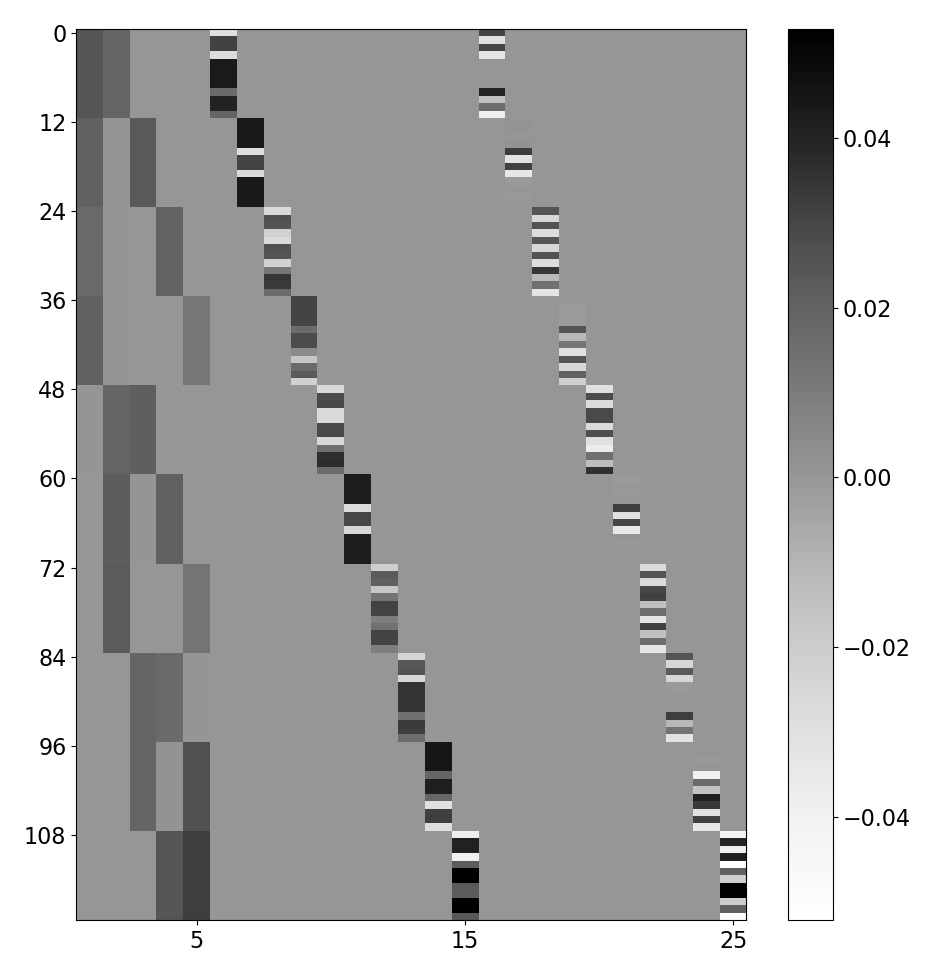
\includegraphics[width=0.9\textwidth]{Figure_Chap3/20221010_V2PM_Pola1_706nm.png}
    \end{subfigure}%
    \begin{subfigure}{0.5\textwidth}
        \centering
        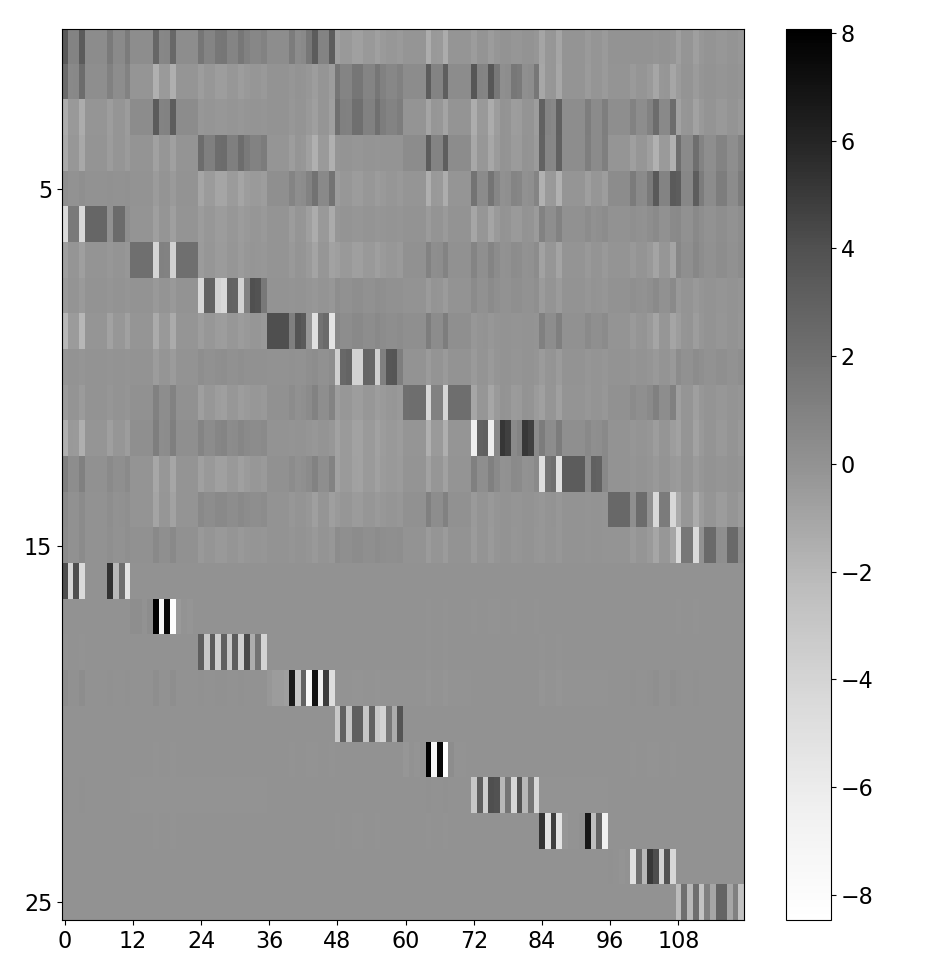
\includegraphics[width=0.9\textwidth]{Figure_Chap3/20221010_P2VM_Pola1_706nm.png}
    \end{subfigure}
    \begin{subfigure}{0.5\textwidth}
        \centering
        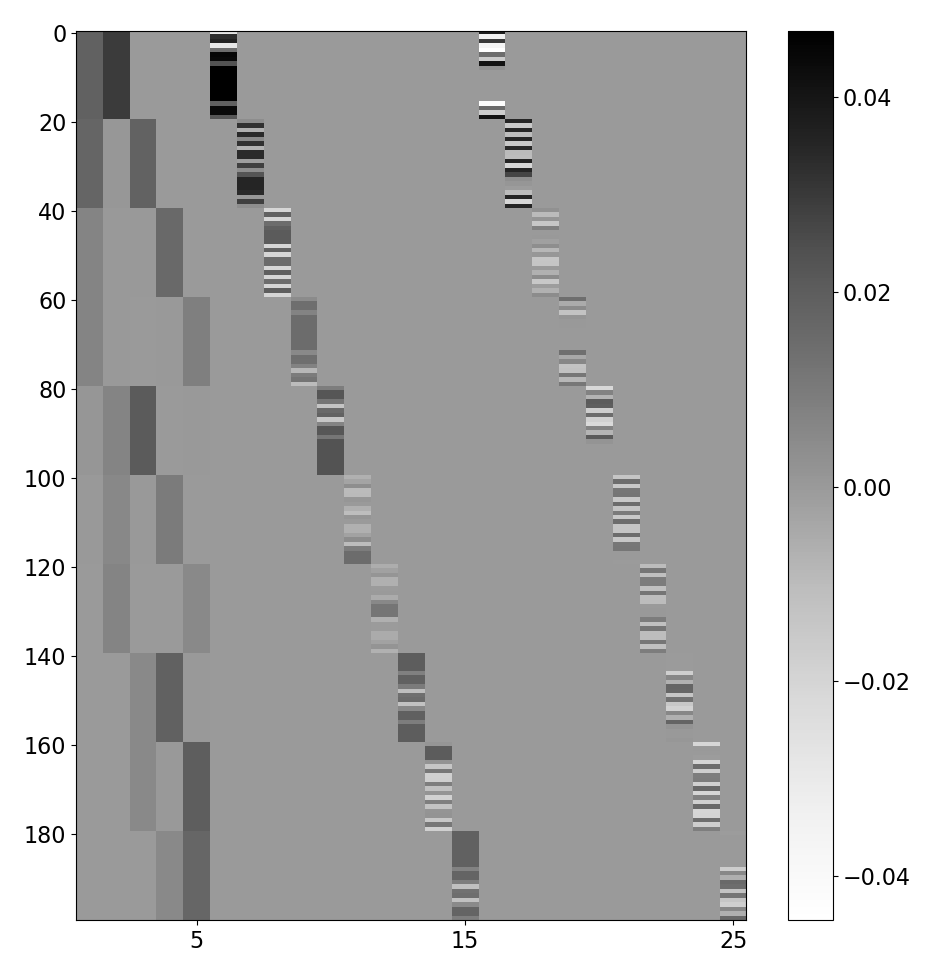
\includegraphics[width=0.9\textwidth]{Figure_Chap3/20220811_V2PM_Pola1_706nm.png}
    \end{subfigure}%
    \begin{subfigure}{0.5\textwidth}
        \centering
        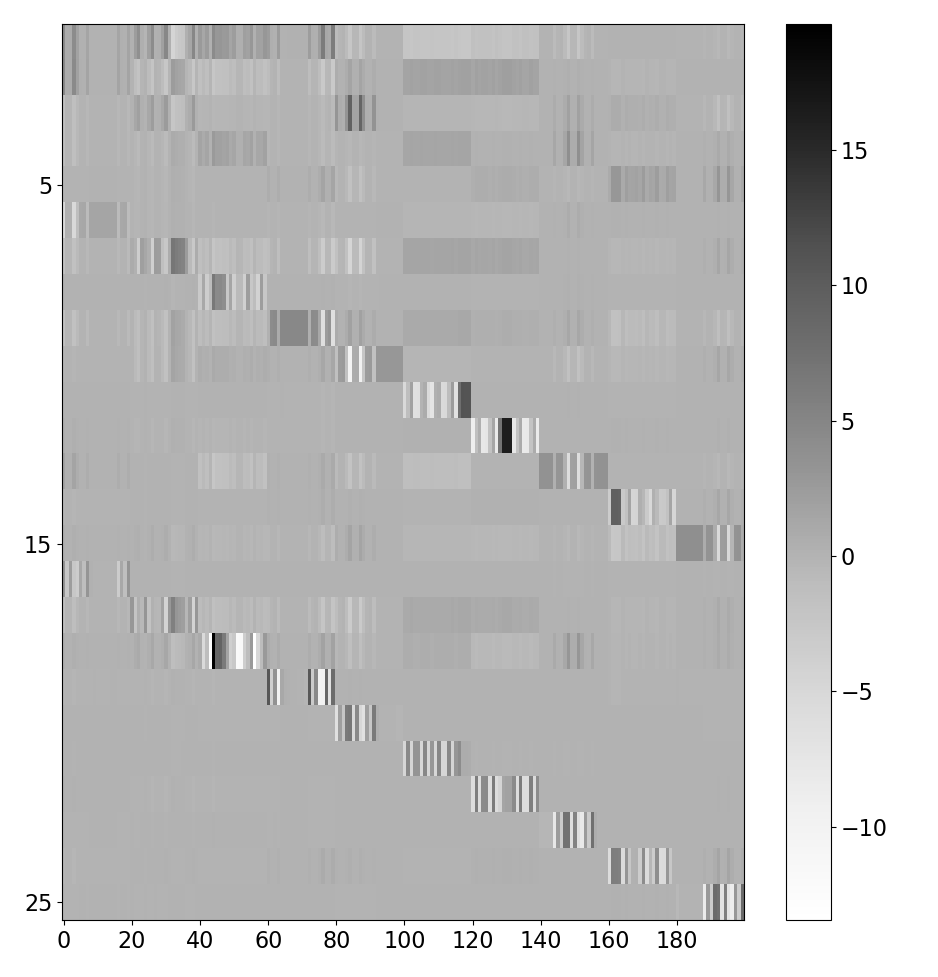
\includegraphics[width=0.9\textwidth]{Figure_Chap3/20220811_P2VM_Pola1_706nm.png}
    \end{subfigure}
    \caption[Représentation graphique de la V2PM et de sa P2VM mesurée sur FIRSTv2, pour les deux puces.]{Représentation graphique de la V2PM (colonne de gauche) et de la P2VM associée (colonne de droite) mesurée sur la puce $Y$ (ligne du haut) et la puce $X$ (ligne du bas). Ce sont les V2PM (P2VM) du canal spectral $\sim 706 \,$nm, mesurées sur FIRSTv2 avec une source \sk. L'axe vertical (respectivement l'axe horizontal) de la V2PM (respectivement de la P2VM) est le nombre de points de la séquence de modulation (OPD) multiplié par le nombre de bases ($12 \times 10 = 120$ pour la $Y$ et $20 \times 10 = 200$ pour la $X$) et l'axe horizontal (respectivement l'axe vertical) contient $5$ termes de transmission en plus de $2 \times 10$ termes interférométriques.}
    \label{fig:V2PMP2VMmesure}
\end{figure}


%%%%%%%%
\subparagraph{Mesure des termes de transmission \\}

Les termes de transmission $E_{n}^2$, arrangés par couple de sous-pupilles,  remplissent les cinq premières colonnes. Pour un paquet de $n_p$ lignes donné (correspondant à une base) les lignes se composent des deux termes $E_{n}^2$ et $E_{n'}^2$ et de zéros. Les bases sont ordonnées, de haut en bas, dans l'ordre des bases $1-2$, $1-3$, $1-4$, $1-5$, $2-3$, $2-4$, $2-5$, $3-4$, $3-5$ et $4-5$, les termes non nuls étant placés dans les colonnes $n$ et $n'$ correspondantes à la base.

Afin d'effectuer leur mesure, cinq séries d'images sont prises en illuminant tour à tour les sous-pupilles. Pour cela, tous les segments sont positionnés en bout de course du tip-tilt sauf le segment de la sous-pupille d'intérêt qui est envoyé sur sa position d'optimisation de l'injection (voir section~\ref{sec:OptiInj}). Ainsi, $4$ ($8$ pour la puce $X$) sorties sont illuminées sur la caméra et une série de quelques centaines d'images est acquise pendant que les segments sont modulés en piston selon la séquence de modulation des franges pour prendre en compte les potentielles variations du flux dans les fibres. La figure~\ref{fig:flats} montre les cinq images obtenues après la moyenne de ces cinq séries, où les sorties sont réparties sur l'axe vertical et la dispersion spectrale sur l'axe horizontal. Les bases sont identifiées sur la caméra en détectant les sorties qui sont illuminées.

\begin{figure}[ht!]
    \begin{subfigure}{\textwidth}
        \centering
        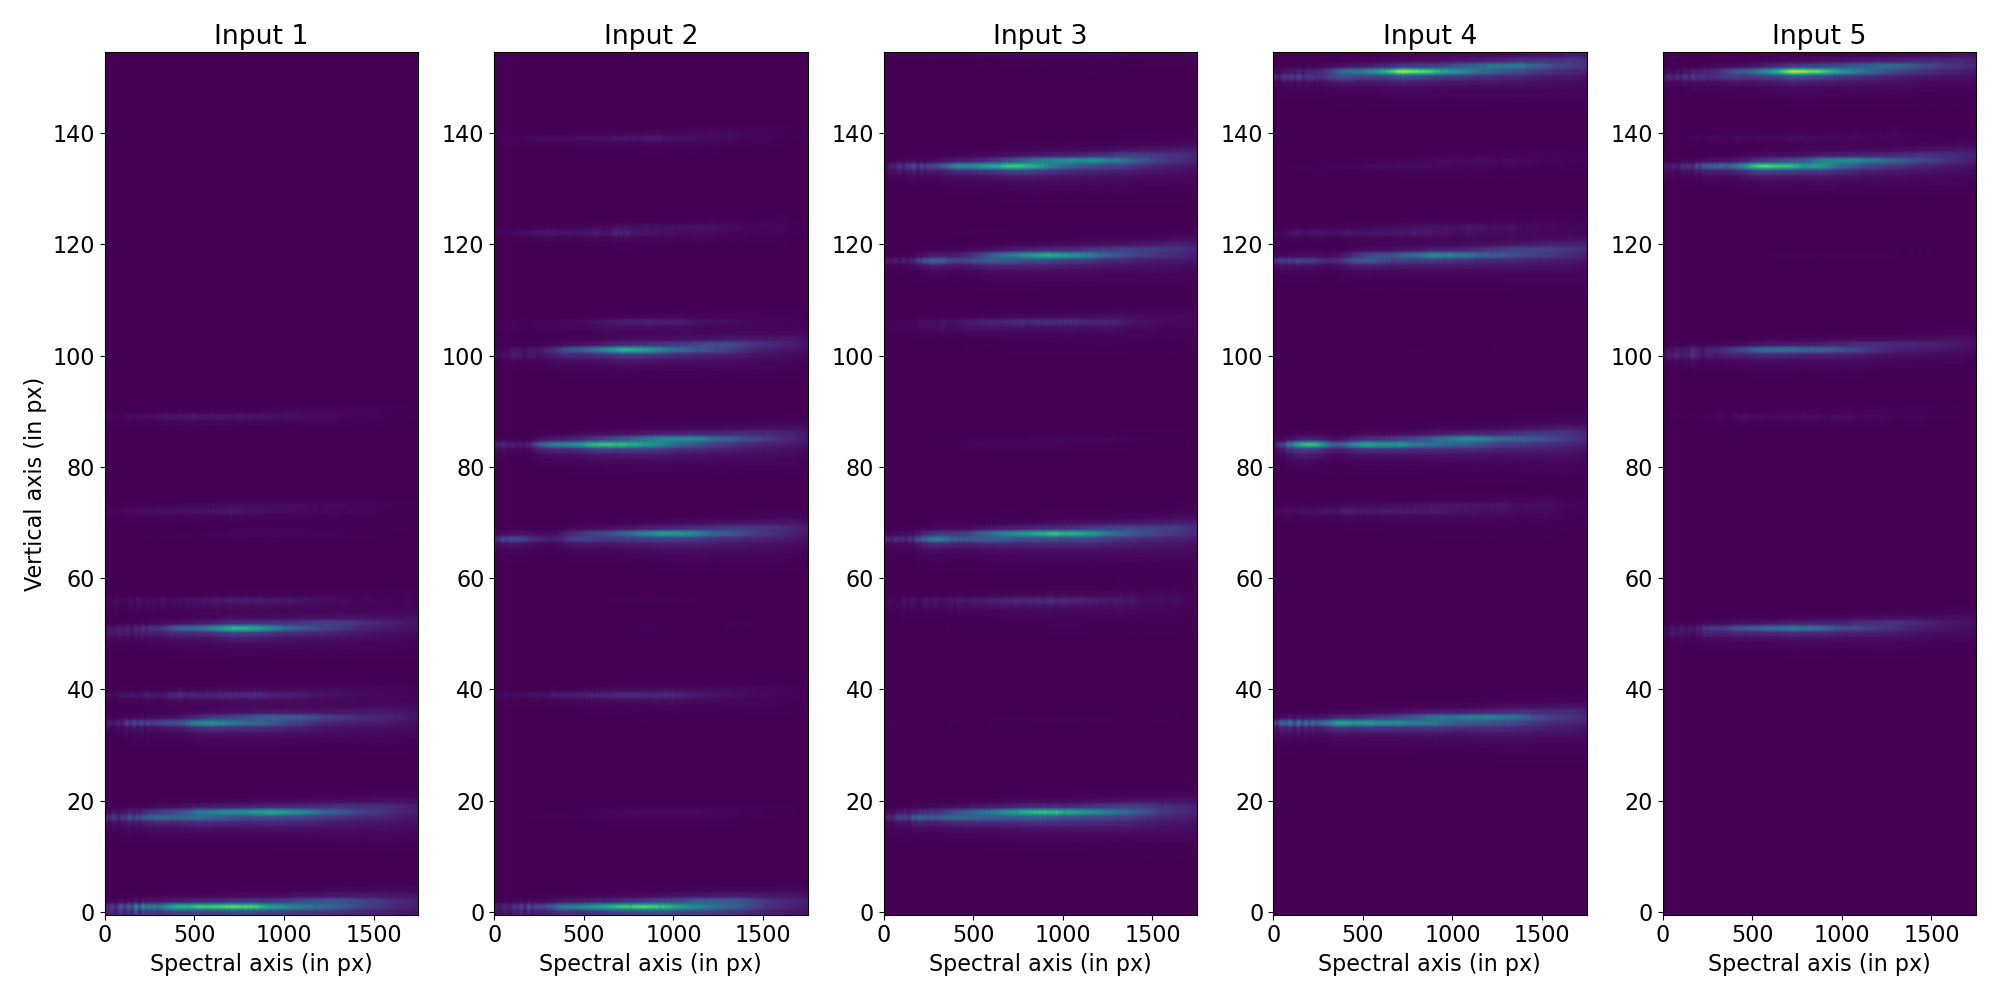
\includegraphics[width=0.8\textwidth]{Figure_Chap3/20221010_Flats.png}
    \end{subfigure}
    \begin{subfigure}{\textwidth}
        \centering
        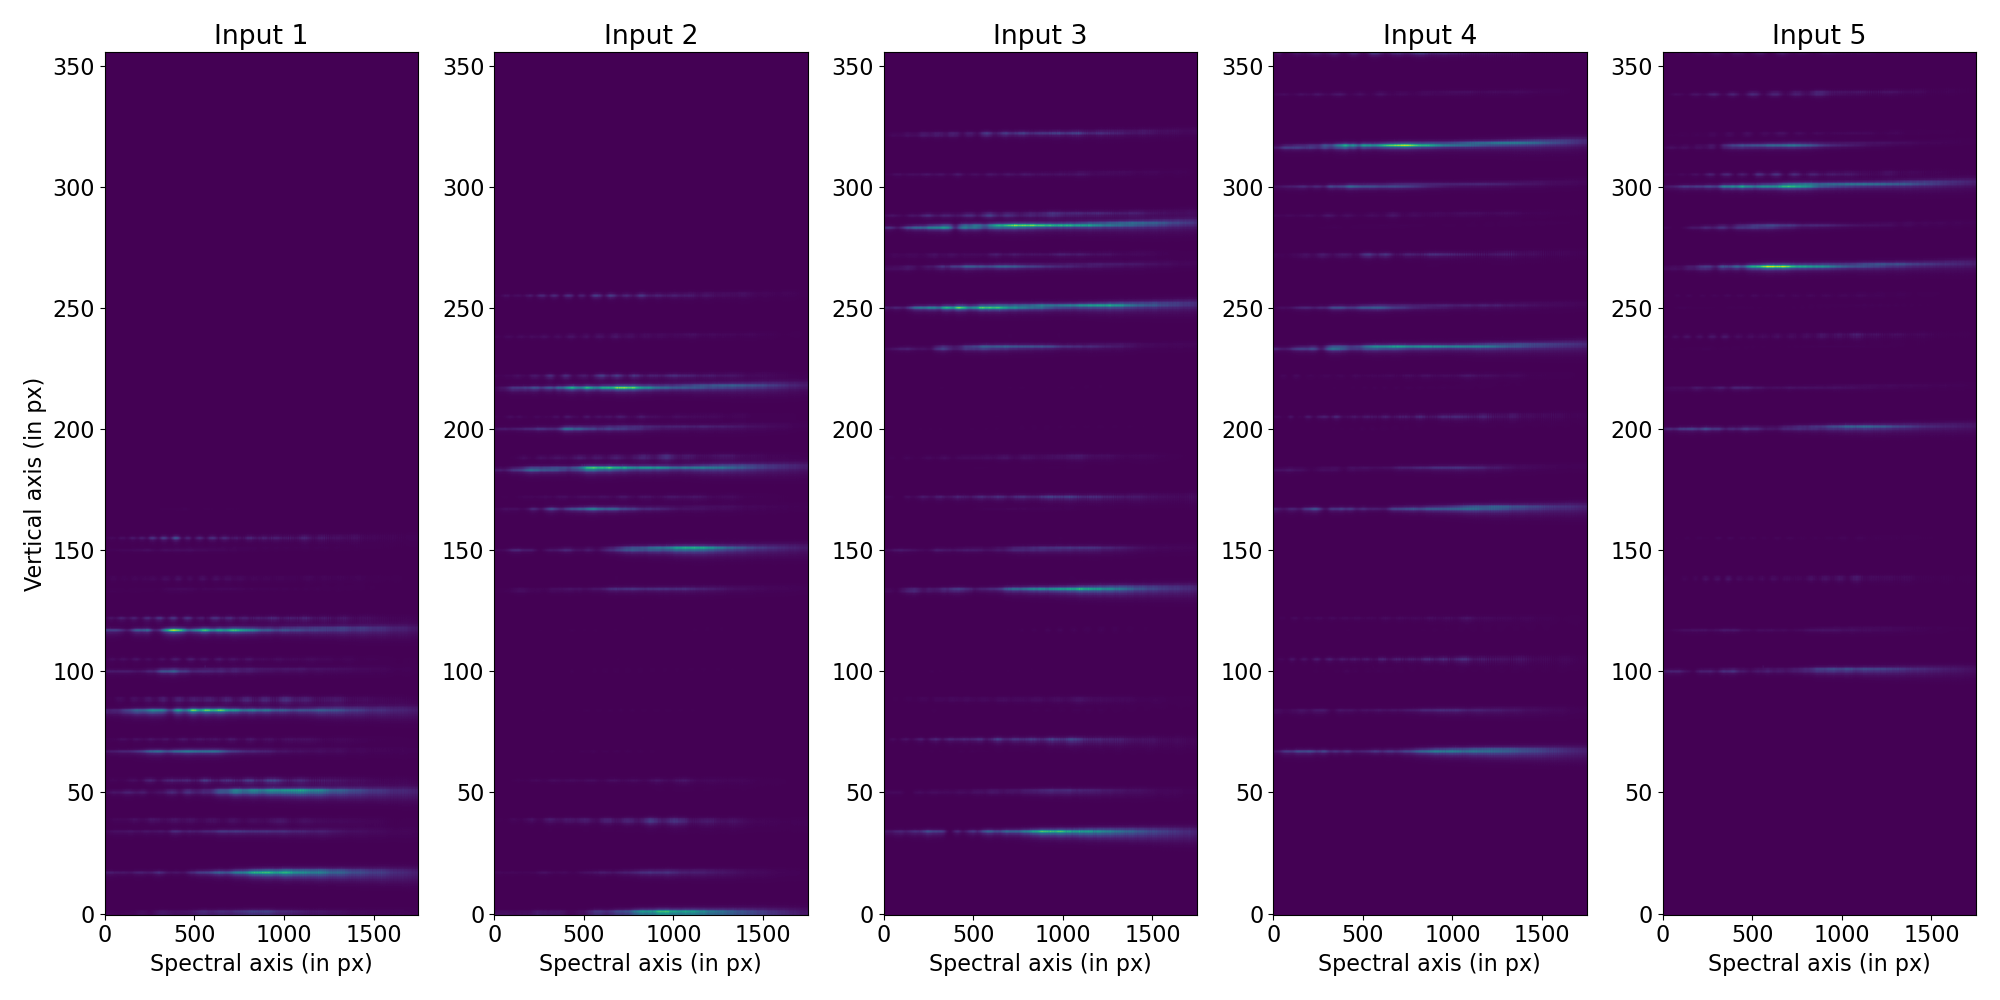
\includegraphics[width=0.8\textwidth]{Figure_Chap3/20220811_Flats.png}
    \end{subfigure}
    \caption[Les flats mesurés sur les deux puces, sur FIRSTv2.]{Les cinq images de la caméra lorsque les entrées de la puce $Y$ (en haut) et de la puce $X$ (en bas) sont individuellement éclairées. Sur chaque image, on peut identifier les $4$ ($8$ pour la puce $X$) sorties selon l'axe vertical et la dispersion spectrale selon l'axe horizontal. On note que sur ces images, le nombre de sorties visibles est en réalité le double à cause de la présence d'un prisme de wollaston sur le chemin optique.}
    \label{fig:flats}
\end{figure}

Pour chaque entrée illuminée, le flux de chaque sortie est normalisé par la somme des flux des $4$ ($8$ pour la puce $X$) sorties illuminées par cette entrée. Et cela est fait pour chaque pas de la séquence de modulation et pour chaque canal spectral. La figure~\ref{fig:V2PMtransmission} présente les spectres de transmission à la suite de cette opération pour les quatre sorties des cinq entrées de la puce $Y$, pour le premier pas de la séquence de modulation. On remarque que les deux courbes, pour une sortie donnée, ne sont pas nécessairement les mêmes selon que la sortie est illuminée par l'une ou l'autre des deux entrées. Cela est dû au fait que chaque sortie est illuminée par deux chemins différents. De plus, la partie inférieure à $640 \,$nm présente de grandes variations par rapport au reste du spectre, car la puce a été spécifiée monomode dans la bande spectrale $650 - 800 \,$nm et ne l'est pas en dehors. Les prochaines puces seront conçues pour être monomodes au minimum dans la gamme spectrale $600 - 700 \,$nm pour être capable de faire des mesures de raie d'émission \ha~à $656.28 \,$nm, ce qui correspond à notre cas scientifique (voir la section~\ref{sec:AccretionAlpha}).

\begin{figure}[ht!]
    \begin{subfigure}{\textwidth}
        \centering
        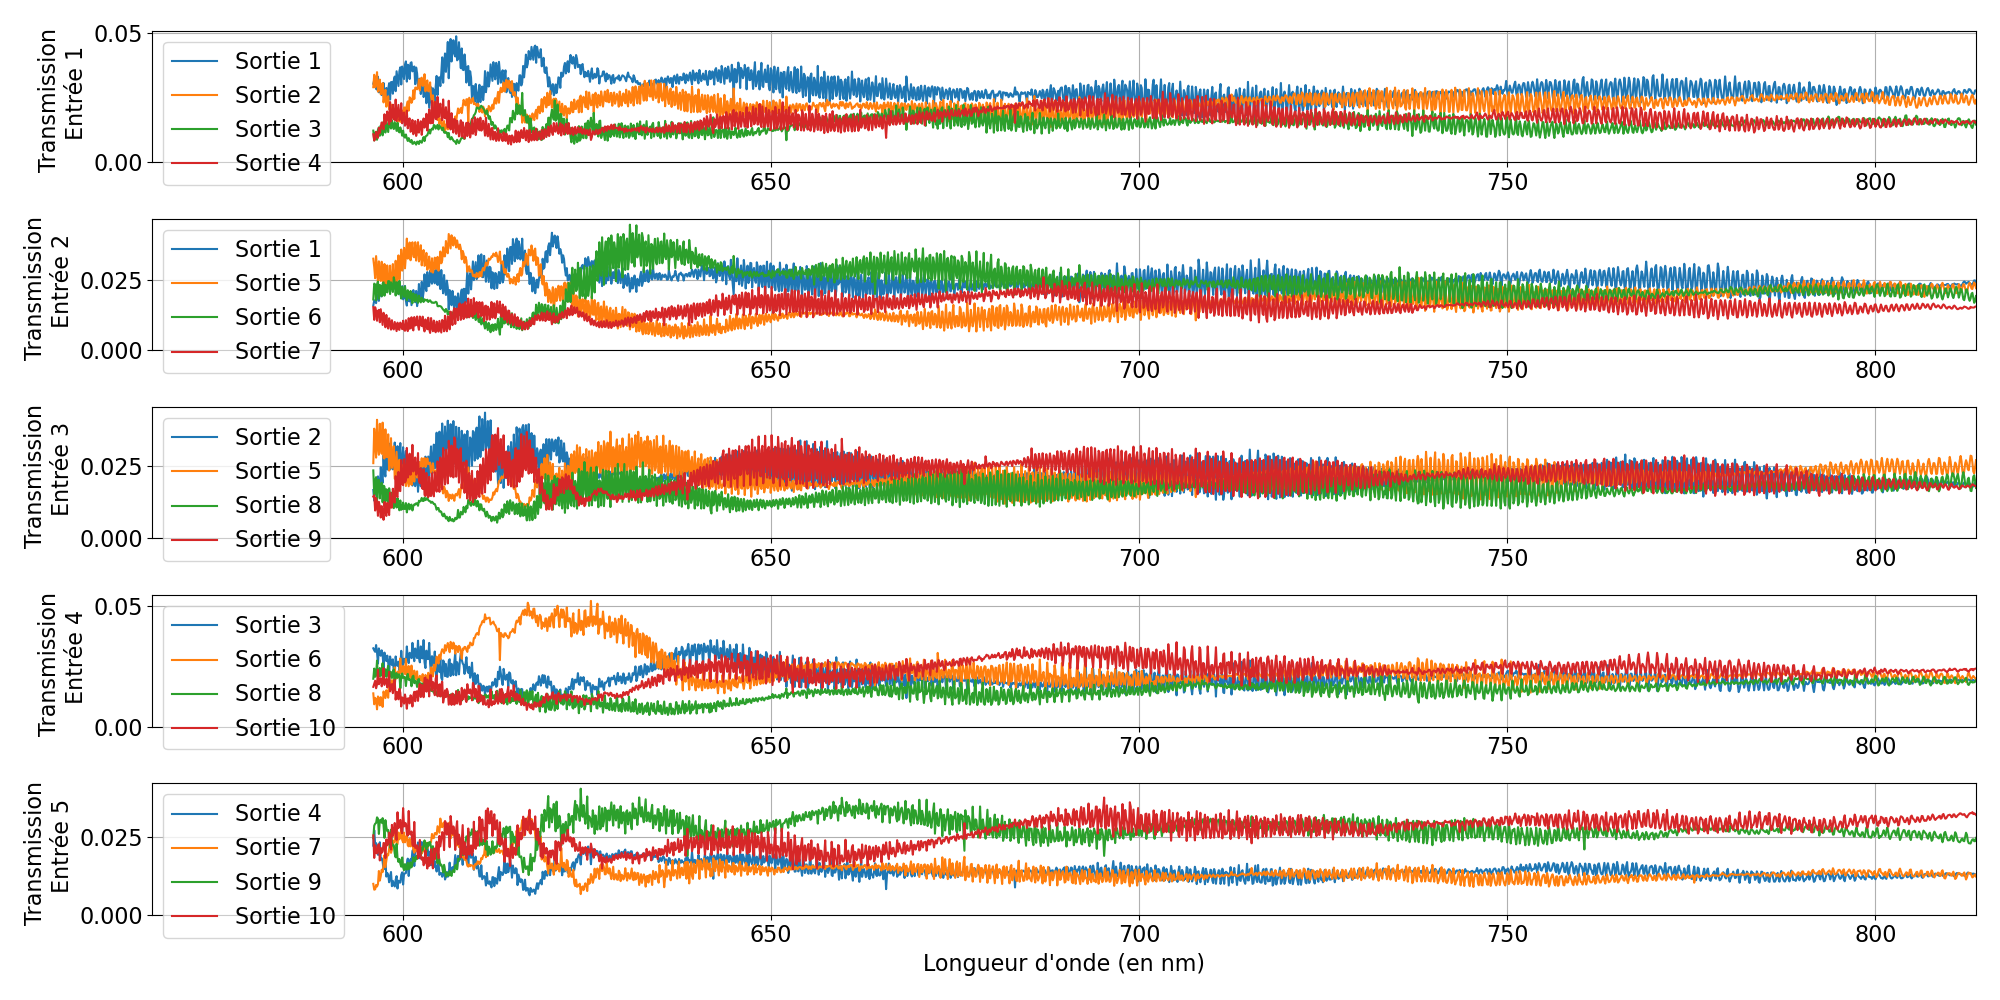
\includegraphics[width=0.8\textwidth]{Figure_Chap3/20221010_P2VM_01_SpectralThroughput.png}
    \end{subfigure}
    \begin{subfigure}{\textwidth}
        \centering
        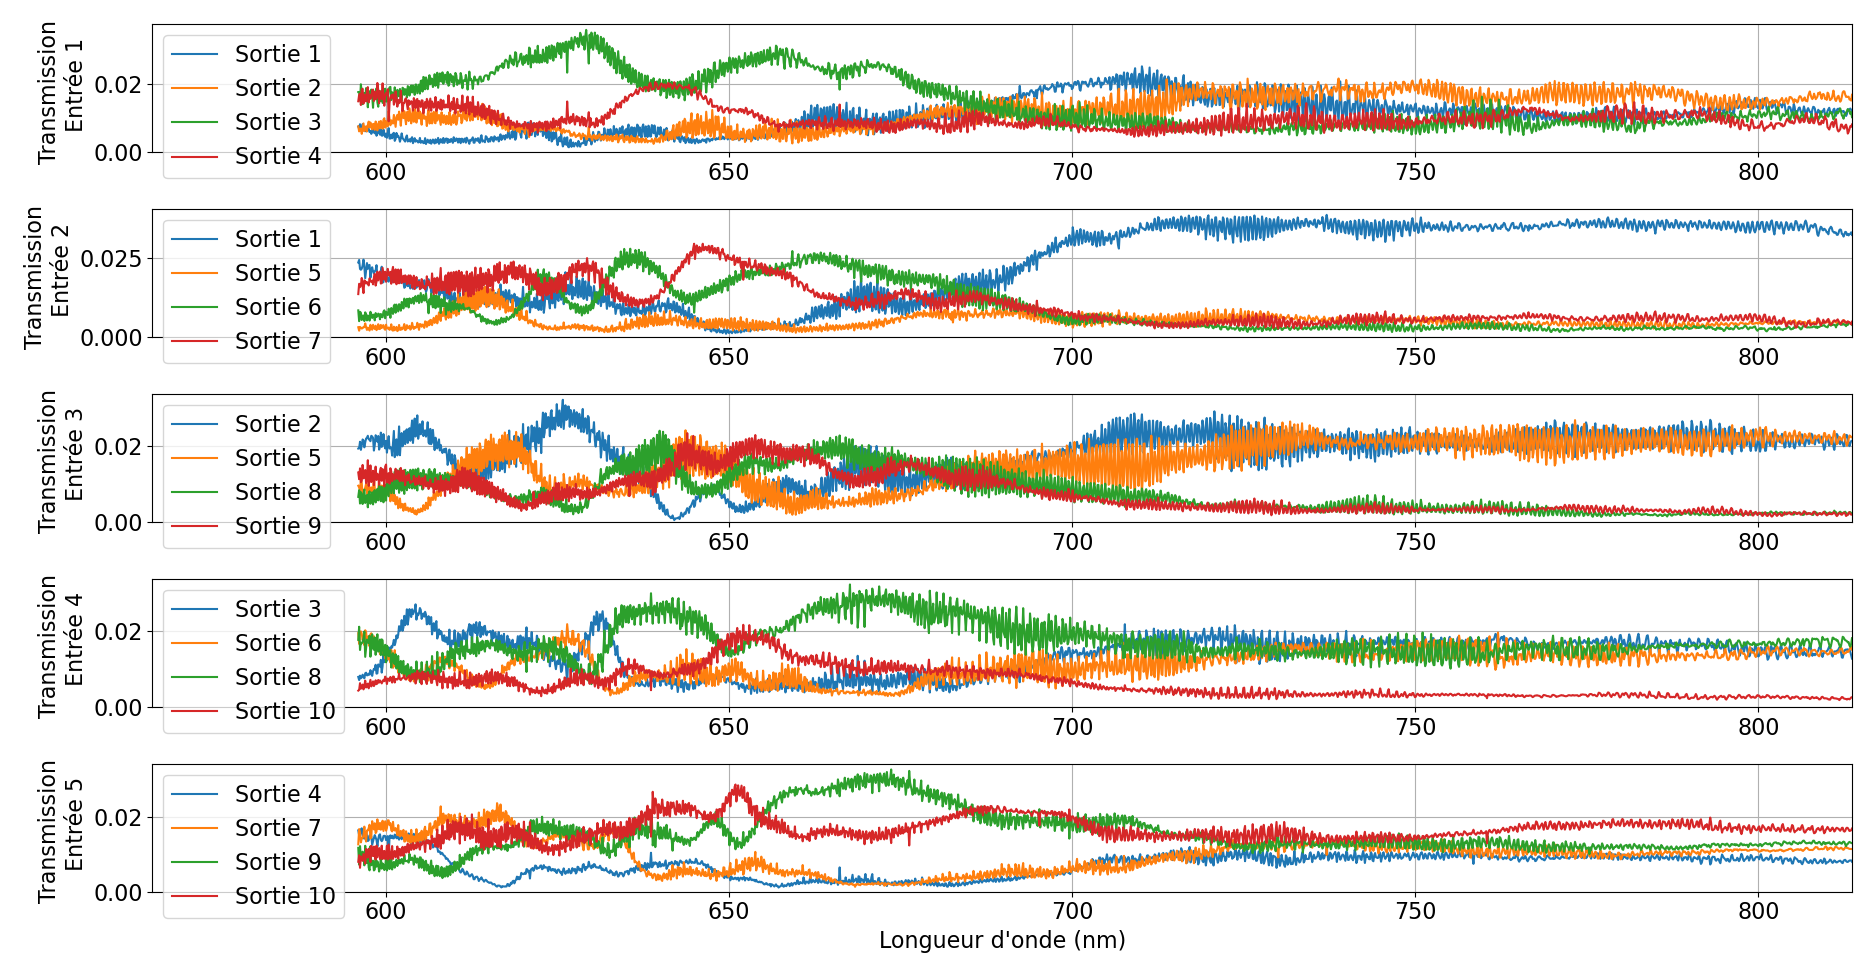
\includegraphics[width=0.8\textwidth]{Figure_Chap3/20220811_P2VM_01_SpectralThroughput.png}
    \end{subfigure}
    \caption[Transmissions relatives mesurées sur chaque entrée des puces $Y$ et $X$, constituant les 5 premières colonnes de la V2PM.]{Les spectres de transmissions relatives pour le premier pas de la séquence de modulation mesurés sur les quatre sorties (voir les légendes) en illuminant une à une les cinq entrées de la puce (de haut en bas). Les cinq graphiques du haut sont les transmissions mesurées avec la puce $Y$ et les cinq du bas avec la puce $X$. Ces courbes remplissent les cinq premières colonnes des V2PMs pour les canaux spectraux correspondant.}
    \label{fig:V2PMtransmission}
\end{figure}


%%%%%%%%
\subparagraph{Mesure des termes interférométriques \\}

Dans cette partie, on souhaite mesurer expérimentalement la séquence de modulation des franges. Pour cela, les interférogrammes sont modulés en phase les uns après les autres et la phase des franges est estimée pour chaque pas de la séquence et remplit les dernières colonnes de la \ac{V2PM}, selon la procédure décrite ci-après.

En effet, on souhaite estimer les termes $C_{b_i}(x)$ et $S_{b_i}(x)$ qui remplissent les vingt dernières colonnes de la \ac{V2PM}. La procédure de l'instrument \ac{AMBER} préconise de mesurer les franges d'interférences indépendamment sur chaque base. Pour cela, seules les entrées $n$ et $n'$ de la puce formant la base $b_i$ sont illuminées et une série d'images est acquise en appliquant la séquence de modulation des franges. Cette acquisition est répétée cinq fois en translatant de manière aléatoire de quelques micromètres les cinq lignes à retard (\acrfull{ODL}) afin de mesurer les interférogrammes sur une plus grande diversité de phase. Il résulte ainsi $5$ séries d'images avec les franges modulées pour chacune des $10$ bases. 

Par la suite, une image est formée à partir des $5$ séries, pour chaque base successivement, en considérant une partie du spectre seulement. Dans l'idéal on ne souhaiterait utiliser qu'un seul canal spectral afin d'estimer la phase de la séquence évaluée à une longueur d'onde donnée. Mais en pratique on choisit de l'ordre de la dizaine de canaux sur la partie du spectre avec le plus de flux (ce qui correspond à une largeur spectrale de $\sim 6\,$nm), afin d'améliorer le \ac{SNR} de l'estimation des phases dans la suite. Cette image est formée en disposant les interférogrammes mesurés ($12$ points) par colonne, donnant une taille d'image de $12$ lignes par $5 \times n_{sm} \times \Delta\lambda_{px}$, $5$ étant le nombre de série d'images acquises, $n_{sm}$ le nombre de séquence de modulation effectuées lors de cette série et $\Delta\lambda_{px} = 50$ le nombre de canaux spectraux utilisés. Pour une série de $400$ images ($20$ acquisitions répétées $5$ fois), la taille de l'image finale est donc de $12$ lignes par $5 \times 33 \times 50 = 8\,250$ colonnes. Une décomposition en valeurs singulières, ou \ac{SVD}, est alors opérée sur cette image afin d'en déduire les vecteurs propres sur lesquels l'image se projette. Comme elle est composée des interférogrammes mesurés, on s'attend à ce que seulement deux vecteurs propres aient des valeurs singulières qui dominent la décomposition. Ces deux vecteurs propres sont orthonormaux et peuvent donc être assimilés aux fonctions cosinus et sinus de l'équation~\ref{eq:InterferogrammeLineaire}. La phase de l'interférogramme est ainsi déduite de l'angle formé par ceux-ci.

La figure~\ref{fig:SVD} illustre le résultat de la \ac{SVD} appliquée aux données qui ont permis d'estimer la \ac{V2PM} de la figure~\ref{fig:V2PMP2VMmesure}. À gauche sont représentées les valeurs singulières pour chaque base (selon les couleurs de la légende), normalisées par rapport à la première et on voit effectivement que les deux premières dominent les autres. Sur la figure de droite sont tracés les deux vecteurs propres associés aux deux premières valeurs singulières, dans le plan complexe et pour chaque base. Dans cette représentation, une frange idéalement échantillonnée formerait un cercle, constitué de points régulièrement espacés. La séquence de modulation a pour but d'échantillonner au mieux ces cercles, avec au minimum $4$ points déphasés de $\uppi / 2 \,$rad (il s'agit de la méthode ABCD, voir la figure~\ref{fig:FringeSamplingABCD}). Or, la séquence de modulation des franges utilisée ne mesure pas seulement ces quatres points, mais elle en mesure quatre autres pour quatre valeurs d'\ac{OPD} différentes (voir la section~\ref{sec:Modulation}). Cela se remarque en comptant le nombre de points tracés sur les graphiques (au nombre de 8 ou de 9 suivant si le point à zéro \ac{OPD} est mesuré ou non). Aussi, les bases 2 et 6 ne présentent que cinq points de mesure, ce qui se comprend en regardant les valeurs d'\ac{OPD} appliquées par la séquence de modulation présentée sur le bas de la figure~\ref{fig:ModSeq12}.

Ces graphes nous ont servi de point de vérification que la \ac{SVD} a bien fonctionné, nous permettant de faire des corrections ou des améliorations du code lui-même ou nous indiquant que le traitement peut poursuivre. Dans le cas où cela ne fonctionne pas et que les deux premières valeurs singulières ne dominent pas les autres ou que les vecteurs propres ne forment pas des cercles (cela peut apparaître comme des ellipses ou des formes non régulières ou non équitablement échantillonnés), cela peut vouloir dire qu'il y a un problème dans la prise de données (e.g. il est arrivé que les segments du \ac{MEMS} soient restés immobiles), dans la séquence de modulation choisie (plusieurs séquences ont été testées) ou dans le processus de réduction de données en amont.

\begin{figure}[ht!]
    \begin{subfigure}{0.5\textwidth}
        \centering
        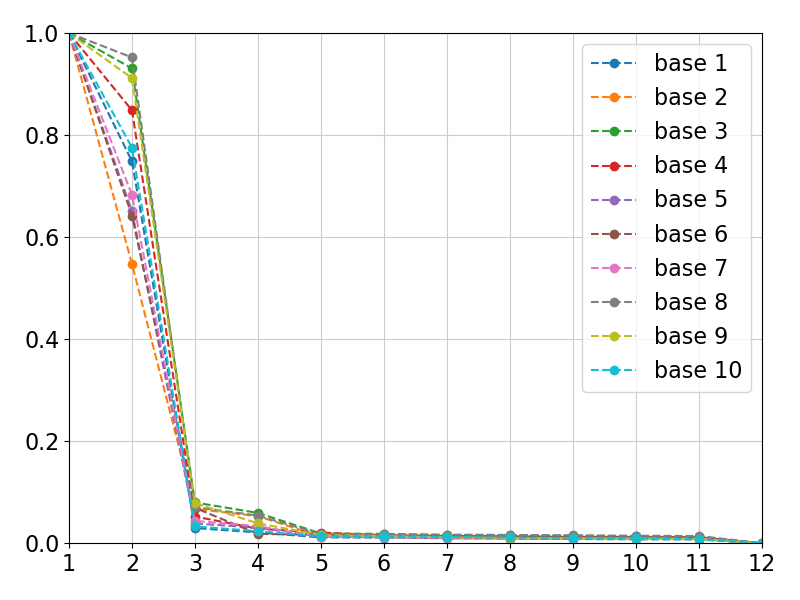
\includegraphics[width=\textwidth]{Figure_Chap3/20221010_SingValue_PolaBase_LaTex.png}
    \end{subfigure}%
    \begin{subfigure}{0.5\textwidth}
        \centering
        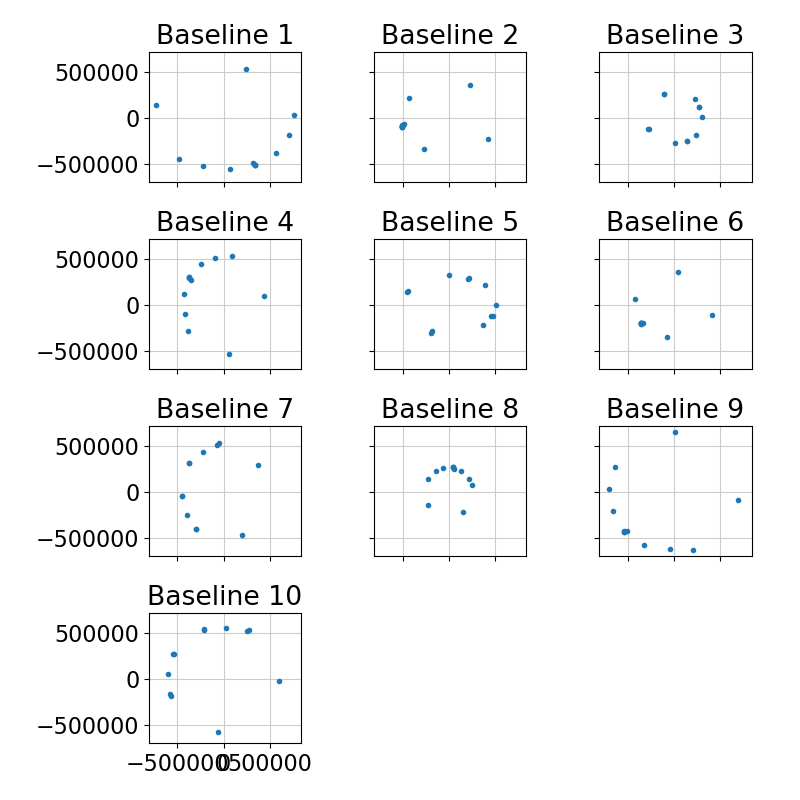
\includegraphics[width=\textwidth]{Figure_Chap3/20221010_ComplexVisibility_Pola1_Base_LaTex.png}
    \end{subfigure}
    \caption[Produits finaux de la SVD appliquée aux données de FIRSTv2 mesurées avec la puce $Y$.]{Produits finaux de la SVD appliquée aux données de FIRSTv2 mesurées avec la puce $Y$. A gauche sont tracées les valeurs singulières trouvées pour chaque base (selon les couleurs de la légende), normalisées par rapport à la première et pour chaque étape de la séquence de modulation en abscisse. A droite sont représentées les vecteurs propres dans le plan complexe.}
    \label{fig:SVD}
\end{figure}

Ensuite, sont déduites les phases pour chaque point de la séquence de modulation à partir de ces deux vecteurs propres. Les \ac{OPD}s $\delta_0$ sont déduites des phases et sont comparées aux \ac{OPD}s théoriques appliquées par la séquence de modulation. Pour cela, la longueur d'onde $\lambda_0$ à laquelle sont mesurées ces phases $\psi_0$ est calculée comme la moyenne des longueurs d'ondes sur les $50$ canaux spectraux choisis. Enfin, les phases $\psi_i$ sur toutes les longueurs d'ondes $\lambda_i$ de la bande spectrale sont obtenues à partir de $\psi_i = 2 \pi \delta_0 / \lambda_i$. Le résultat est tracé sur la figure~\ref{fig:PhaseEstimees}, pour chaque base, où la phase attendue est tracée en trait continu noir et la phase estimée est tracée en trait discontinue bleue, ici pour la longueur d'onde $\sim 706 \,$nm. On voit que les phases sont correctement estimées par rapport à celles attendues. Finalement, ces phases forment les termes de visibilité complexe dont les parties réelles et imaginaires remplissent les $20$ dernières colonnes d'autant de \ac{V2PM} qu'il y a de canaux spectraux, selon le système d'équations~\ref{eq:V2PMtermesComplexes}.

\begin{figure}[ht!]
    \centering
    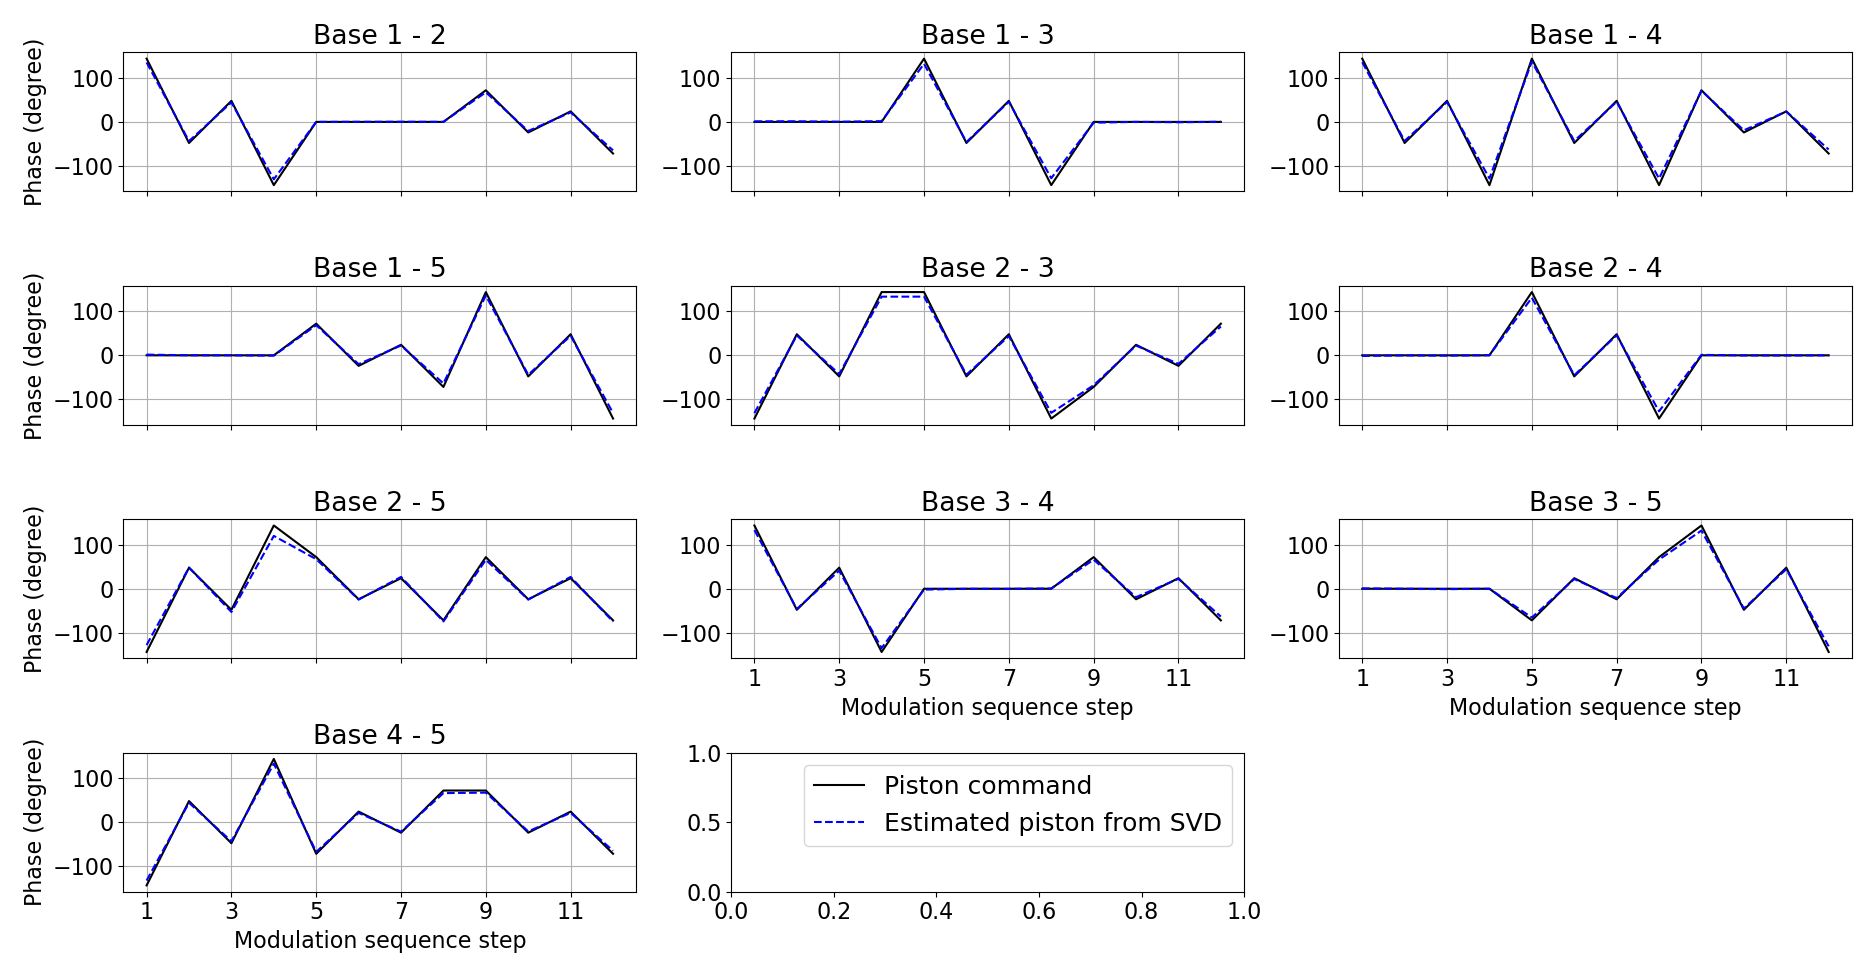
\includegraphics[width=\figwidth]{Figure_Chap3/20221010_ModSeq_L874_EstPhase830_880_Pola1_Base_LaTex.png}
    \caption[Phases estimées par la SVD comparées aux phases attendues en fonction des pas de la séquence de modulation.]{Phases estimées par la SVD comparées aux phases attendues en fonction des pas de la séquence de modulation, sur la puce $Y$. Pour chaque base, les phases attendues, induites par les pistons appliqués sur le MEMS, sont tracées en trait continu noir et les phases estimées sont tracées par dessus en trait discontinu bleu. Ces graphiques sont tracés pour la longueur d'onde $\sim 706 \,$nm.}
    \label{fig:PhaseEstimees}
\end{figure}


%%%%%%%%%%%%%%%%
% \subsection{Estimation du contraste interférométrique}
% les premiers termes de la V2PM
% comparaison pour les 2 puces
% comparaison avec le contraste obtenu dans la caractérisation des puces (section précédente)


%%%%%%%%%%%%%%%%%%%%%%%%%%%%%%%%
\section{Ajustement des franges}
\label{sec:FullOnFit}

Maintenant que la \ac{V2PM} est estimée, il s'agit de faire l'acquisition d'images contenant toutes les bases modulées en phase simultanément. La figure~\ref{fig:FullOnData} présente les interférogrammes mesurés pour la puce $Y$ et la puce $X$ sur les lignes d'images $1$ et $3$, respectivement (pour le canal spectral $\sim 706 \,$nm). Chaque colonne d'images est associée à une base et chaque image est une matrice de dimension $n_p \times n_S$ avec $n_p$ le nombre de points échantillonnés par base en fonction de l'\ac{OPD} (correspondant à une séquence de modulation) et $n_S$ le nombre de fois que la séquence de modulation a été acquise (les interférogrammes sont en fait empilés verticalement). On dispose ainsi de ces matrices pour chaque canal spectral et elles sont ensuite chacune multipliées par la \ac{P2VM} du canal spectral correspondant selon l'équation~\ref{eq:VisibiliteMes}. Le résultat sont les matrices des visibilités $\text{\textbf{P}}$, de dimensions $25 \times n_S$ pour cinq sous-pupilles considérées (et dix bases). On a alors pour chaque base (et chaque canal spectral) le terme de visibilité complexe selon l'équation~\ref{eq:mu}, dans lequel est inclus le terme de piston différentiel intrinsèque à l'instrument, $\psi_{nn'}$. Nous verrons dans la section~\ref{sec:PhaseSpecDiff} comment extraire le terme de phase associée à l'objet observé $\varphi_{nn'}$.

\begin{figure}[ht!]
    \begin{subfigure}{\textwidth}
        \centering
        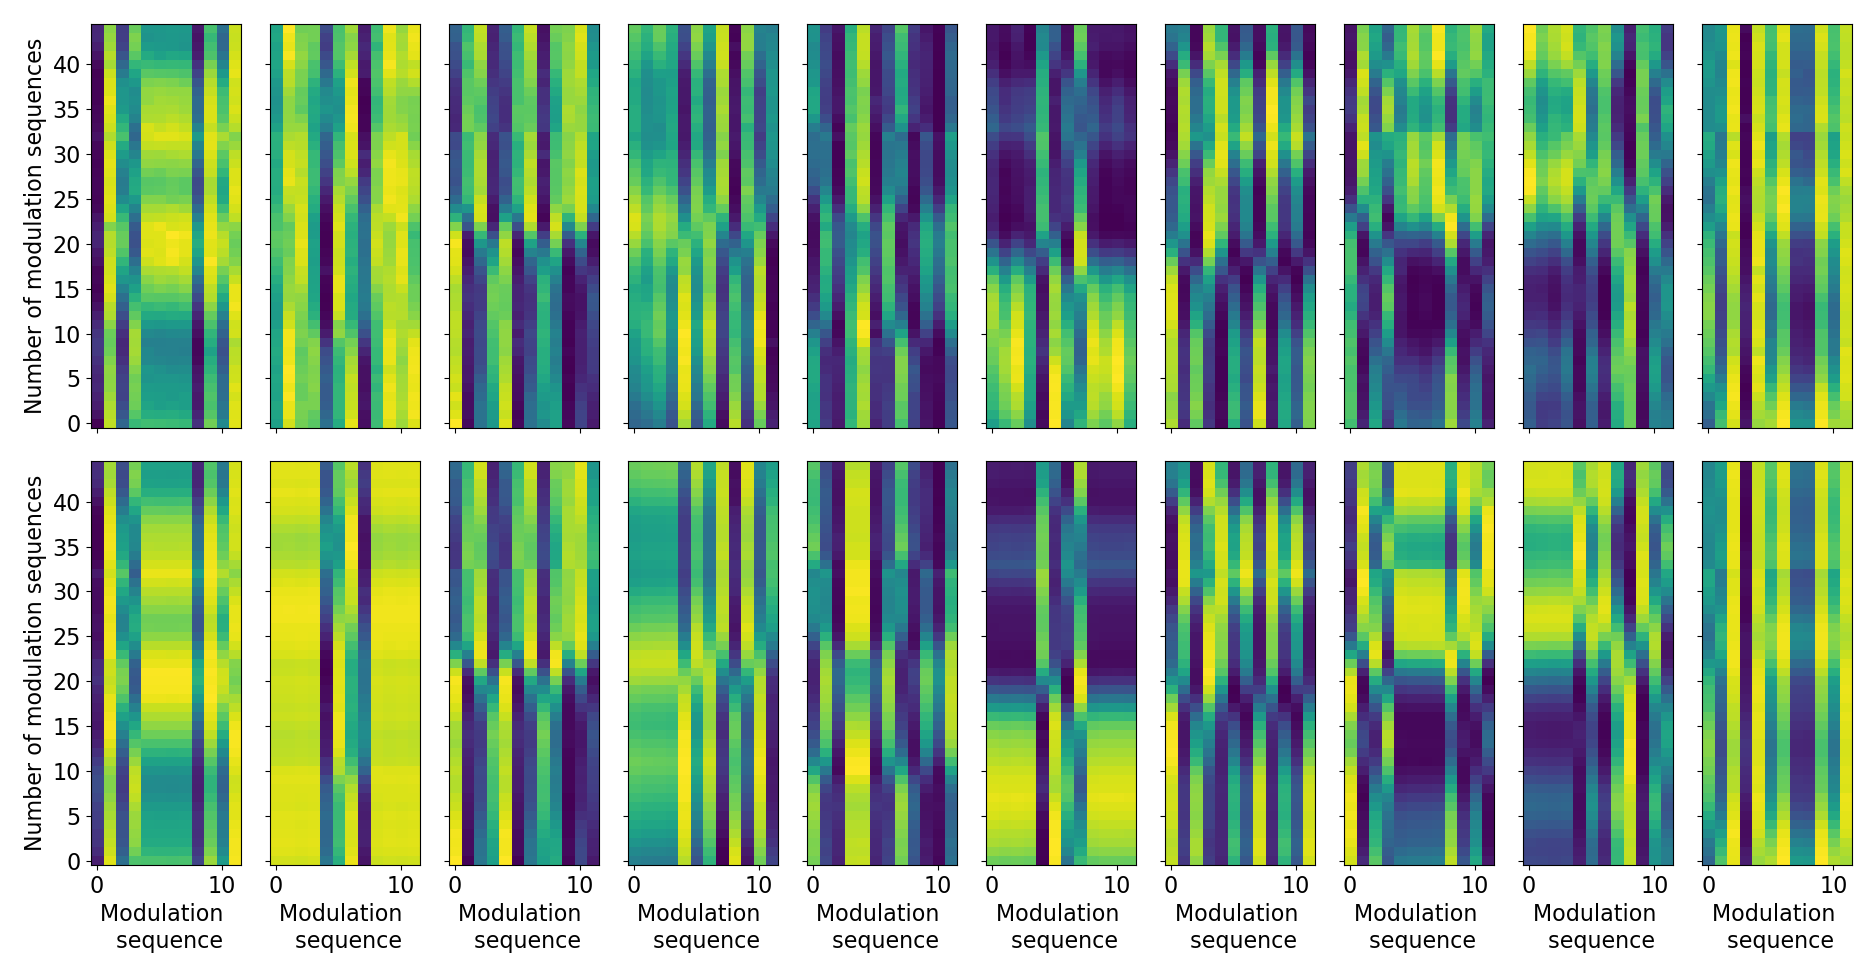
\includegraphics[width=0.9\textwidth]{Figure_Chap3/20221010_FringeFitting_TemporalModulation_Pola1_Base_LaTex.png}
    \end{subfigure}
    \begin{subfigure}{\textwidth}
        \centering
        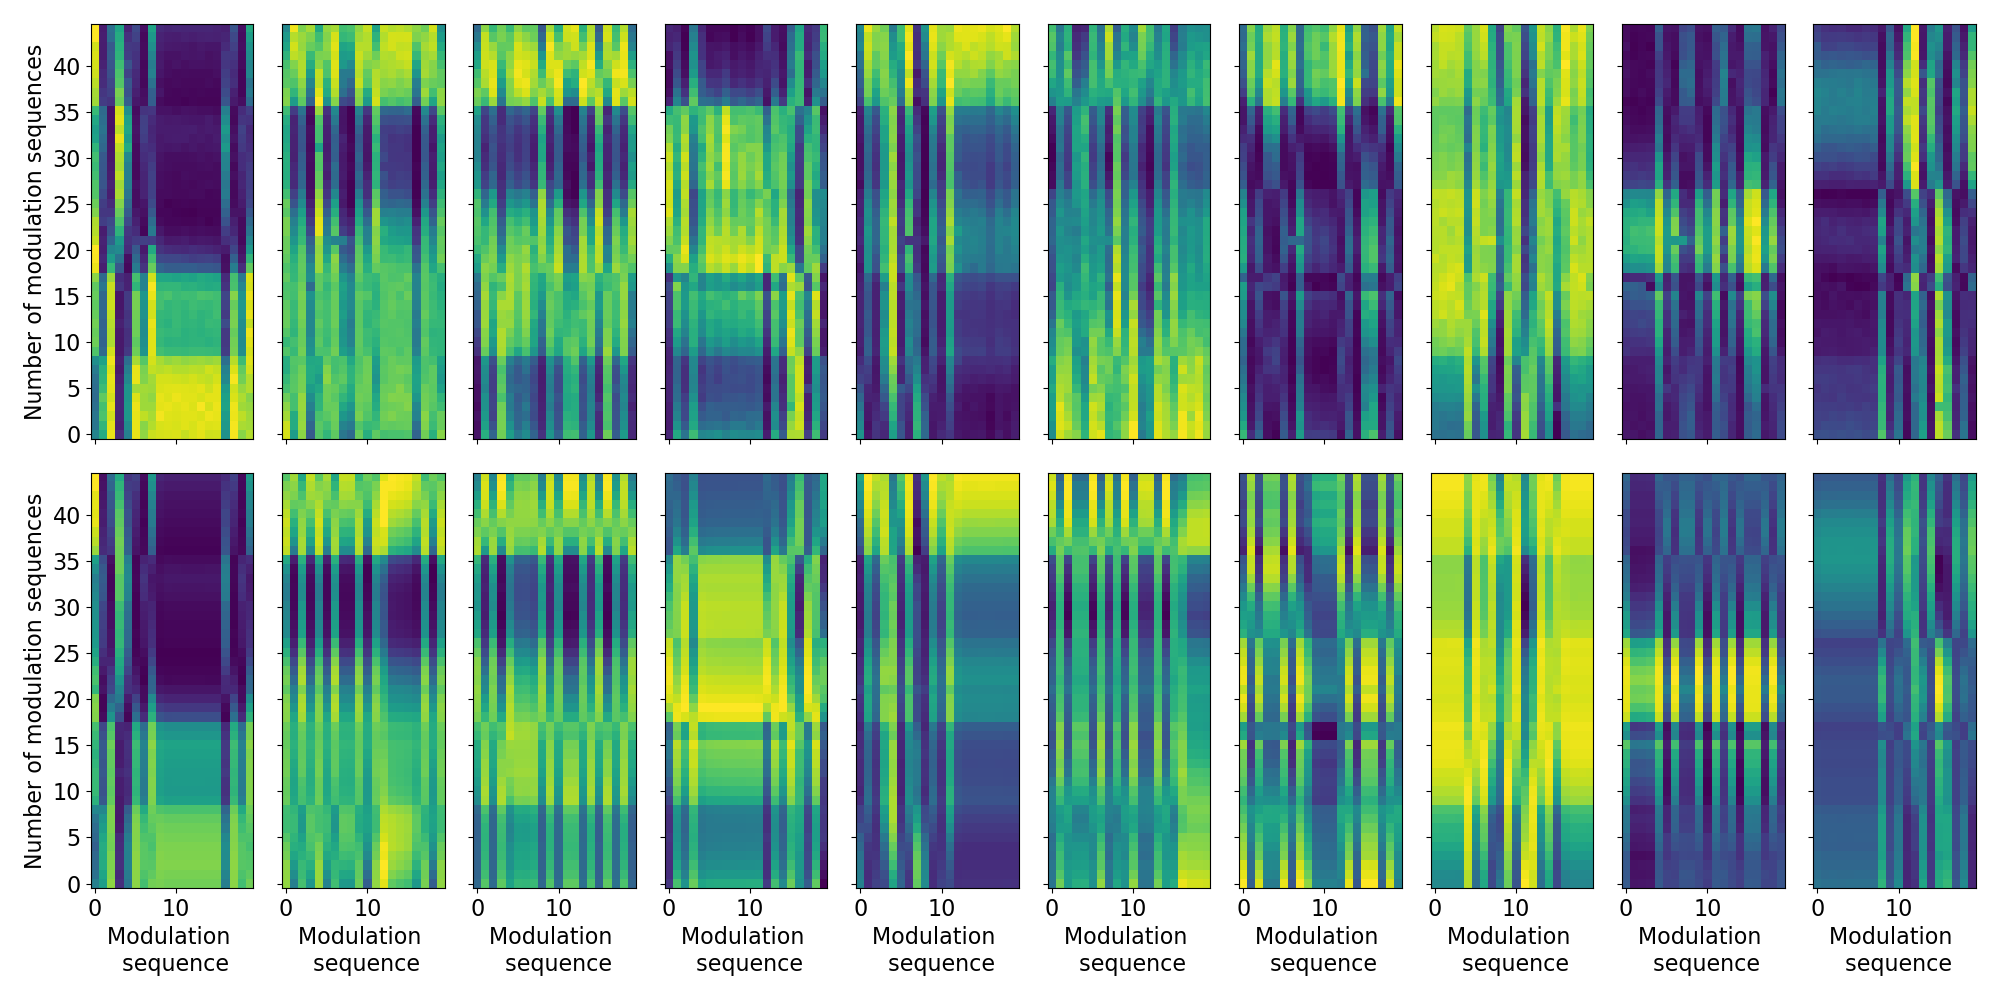
\includegraphics[width=0.9\textwidth]{Figure_Chap3/20220811_FringeFitting_TemporalModulation_Pola1_Base_LaTex.png}
    \end{subfigure}
    \caption[Interférogrammes mesurés et ajustés par la P2VM des puces $Y$ et $X$ mesurés sur FIRSTv2.]{Images des interférogrammes mesurés (lignes du haut) et ajustés (lignes du bas) sur les $10$ bases (en colonne), pour la puce $Y$ (les deux premières lignes) et la puce $X$ (les deux dernières lignes). L'axe horizontal est composé des $12$ et $20$ pas des séquences de modulation pour la puce $Y$ et la puce $X$, respectivement. Les axes verticaux sont le nombre de fois que la séquence de modulation a été acquise. Ces images sont normalisées et sont pour le canal spectral $\sim 706 \,$nm.}
    \label{fig:FullOnData}
\end{figure}

En multipliant la matrice des visibilités $\text{\textbf{P}}$ par la \ac{V2PM} selon l'équation~\ref{eq:FullOnFit}, on reconstruit l'ajustement des interférogrammes mesurés $I_r$. Les lignes d'image $2$ et $4$ de la figure~\ref{fig:FullOnData} sont les ajustements des interférogrammes des lignes $1$ et $3$, respectivement pour la puce $Y$ et la puce $X$.

\begin{equation}
    I_r = V2PM \cdot \text{\textbf{P}} \label{eq:FullOnFit}
\end{equation}

On note que sur tous ces interférogrammes on peut reconnaître la séquence de modulation en s'attardant sur les variations d'intensité selon l'axe horizontal des interférogrammes mesurés de la figure~\ref{fig:FullOnData}, en comparant chaque image de celle-ci à chaque ligne des séquences appliquées des figure~\ref{fig:ModSeq12} et figure~\ref{fig:ModSeq20}.


%%%%%%%%%%%%%%%%%%%%%%%%%%%%%%%%
\section{La phase différentielle spectrale : une observable auto-étalonnée}
\label{sec:PhaseSpecDiff}
% (gravity \citep{amorim2020}) mesure de la masse du trou noir central de la galaxie active IRAS 09149-6206 avec la phase différentielle

%%%%%%%%%%%%%%%%
\subsection{Estimation de la phase différentielle}

La phase différentielle spectrale est une observable auto-étalonnée des erreurs et biais de phase instrumentaux qui s'ajoutent à la phase inhérente à la source astrophysique lors de la mesure. Pour l'obtenir, on utilise le fait que la phase est mesurée en fonction de la longueur d'onde. Le concept de base \citep{buscher2015} est de soustraire la moyenne de la phase sur deux canaux spectraux $\lambda_0 - \Delta\lambda$ et $\lambda_0 + \Delta\lambda$ à la phase du canal spectral central $\lambda_0$. Trois mesures sont donc requises a minima. Dans notre cas, nous disposons de bien plus de canaux spectraux, ce qui permet de modéliser plus finement le continuum.

En pratique, on explicite l'expression de la phase mesurée en fonction du nombre d'onde $\sigma = 1 / \lambda$ pour mettre en évidence les erreurs de phase instrumentales, comme cela a été fait pour le traitement des données d'\ac{AMBER} \citep{millour2008} mais aussi de l'instrument \ac{GRAVITY} \citep{lapeyrere2014}. Premièrement, la phase de l'objet astrophysique peut être développée selon :

\begin{equation}
    \varphi^{ob}_{nn'}(\sigma) = a^{ob}_0 + a^{ob}_1 \sigma + \delta\varphi^{ob}_{nn'}(\sigma) \label{eq:PhaseSource}
\end{equation}

\noindent où $\delta\varphi^{ob}_{nn'}(\sigma)$ est la phase de l'objet qui ne peut pas être exprimée par une pente de phase et qu'on cherche à mesurer : la raie d'émission d'une protoplanète ou une composante en rotation comme cela a été mesuré par l'instrument \ac{GRAVITY} sur le quasar 3C 273 \citep{sturm2018} et sur le trou noir central de la galaxie active IRAS 09149-6206 \citep{amorim2020}.

De plus, l'atmosphère ajoute un terme de phase $\varphi^{atmos}_{nn'}(t, \sigma)$ via une différence de marche achromatique (appelée piston) $p_{nn'}(t)$ s'exprimant :

\begin{equation}
    \varphi^{atmos}_{nn'}(t, \sigma) = 2\pi p_{nn'}(t) \sigma
\end{equation}

Les lignes à retard compensent des différences de longueur de chemin optique dans le verre des fibres optiques en ajoutant une longueur de chemin optique dans l'air. La dépendance spectrale de l'indice de réfraction implique que cette compensation ne peut se faire que pour une longueur d'onde et induit un terme de dispersion chromatique (voir la section~\ref{sec:PhaseDiffFIRSTv2}) noté $\varphi^{disp}_{nn'}(\sigma^2)$.
% \kevinco{pour la dispersion quadratique, peut-on l'exprimer comme dans lacour2014 (section 5.2) ? $D(l1, l2) = delta_air * (n^{l1}_{air} - n^{l2}_{air}) + delta_fibre * (n^{l1}_{fibre} - n^{l2}_{fibre})$ d'où dans nos phases mesurées le terme $(2 pi D(1/l)) / l, en sigma**2$ ?}

Aussi, un terme de phase inhérent à l'instrument est mesuré, de différence de marche $\delta_{nn'}$ et la phase mesurée $\varphi^{m}_{nn'}(t, \sigma)$ s'écrit finalement :

\begin{align}
    \varphi^{m}_{nn'}(t, \sigma) &= \varphi^{ob}_{nn'}(\sigma) + 2\pi\delta_{nn'}\sigma + \varphi^{atmos}_{nn'}(t, \sigma) + \varphi^{disp}_{nn'}(\sigma)\\
    &= a^{ob}_0 + 2\pi(a^{ob}_1 + \delta_{nn'} + p_{nn'}(t)) \sigma + \varphi^{disp}_{nn'}(\sigma^2) + \delta\varphi^{ob}_{nn'}(\sigma)\label{eq:phasefit}
\end{align}

La phase différentielle $\delta\varphi^{m}_{nn'}(\sigma)$ s'obtient par la soustraction de la phase mesurée à une longueur d'onde de travail $\lambda_{work} = 1 / \sigma_{work}$ par la phase mesurée à une longueur d'onde de référence $\lambda_{ref} = 1 / \sigma_{ref}$. Pour cela, on calcule l'argument du produit inter-spectral de la cohérence complexe dans ces deux canaux spectraux :

\begin{equation}
	\delta\varphi^{m}_{nn'}(\sigma) = arg \left ( \langle \mu_{nn'}(t, \sigma_{work}) \mu_{nn'}(t, \sigma_{ref})^* \rangle_t \right ) = \delta\varphi^{ob}_{nn'}(\sigma)
\end{equation}


%%%%%%%%%%%%%%%%
\subsection{En pratique sur FIRSTv2}
\label{sec:PhaseDiffFIRSTv2}

Les canaux spectraux de référence sont définis par toute la bande spectrale en excluant les canaux spectraux de travail. Pour un signal mesuré sur une protoplanète en accrétion qui présente une forte raie d'émission \ha~(voir la section~\ref{sec:Protoplanetes}), les canaux spectraux de travail sont ceux englobant la longueur d'onde \ha. Le signal de phase sur les canaux spectraux de référence correspond au signal du continuum non résolu par l'instrument (l'étoile centrale) et il est nul. Par conséquent, le signal qu'on mesure effectivement sur les canaux spectraux de référence est égal à la phase provenant des pistons atmosphériques et instrumentaux et son ajustement permet de le corriger par interpolation sur les canaux de travail.

On ajuste donc une fonction polynomiale du second degré aux mesures de phases sur les canaux spectraux de référence, image par image (selon la variable $t$), afin de déterminer la fonction de l'équation~\ref{eq:phasefit}. La soustraction de cette fonction ajustée aux phases mesurées sur toute la bande spectrale permet de mettre en évidence le signal provenant uniquement de la protoplanète résolue, correspondant au terme de hauts ordres $\delta\varphi^{*}_{nn'}(\sigma)$ dans l'équation~\ref{eq:PhaseSource} de la phase de la source.

La figure~\ref{fig:FitPhaseVis} présente une telle procédure sur des données prises sur une source binaire (comme expliqué dans la section~\ref{sec:SystBinaire}). Pour chaque base (identifiée dans les sous-titres par \textit{B\#}), un graphique présente les phases des visibilités mesurées en vert et son ajustement en trait discontinu rouge en fonction du nombre d'onde $\sigma = 1/ \lambda$. Le signal du compagnon est entre $0.0015$ et $0.0016 \, \text{nm}^{-1}$ sur les courbes vertes, mais est faible et difficile à voir. La fonction polynomiale trouvée par ajustement est écrite dans le sous-titre de chaque graphique. On note que les phases sont quadratiquement très dépendantes du nombre d'onde.

\begin{figure}[ht!]
    \centering
    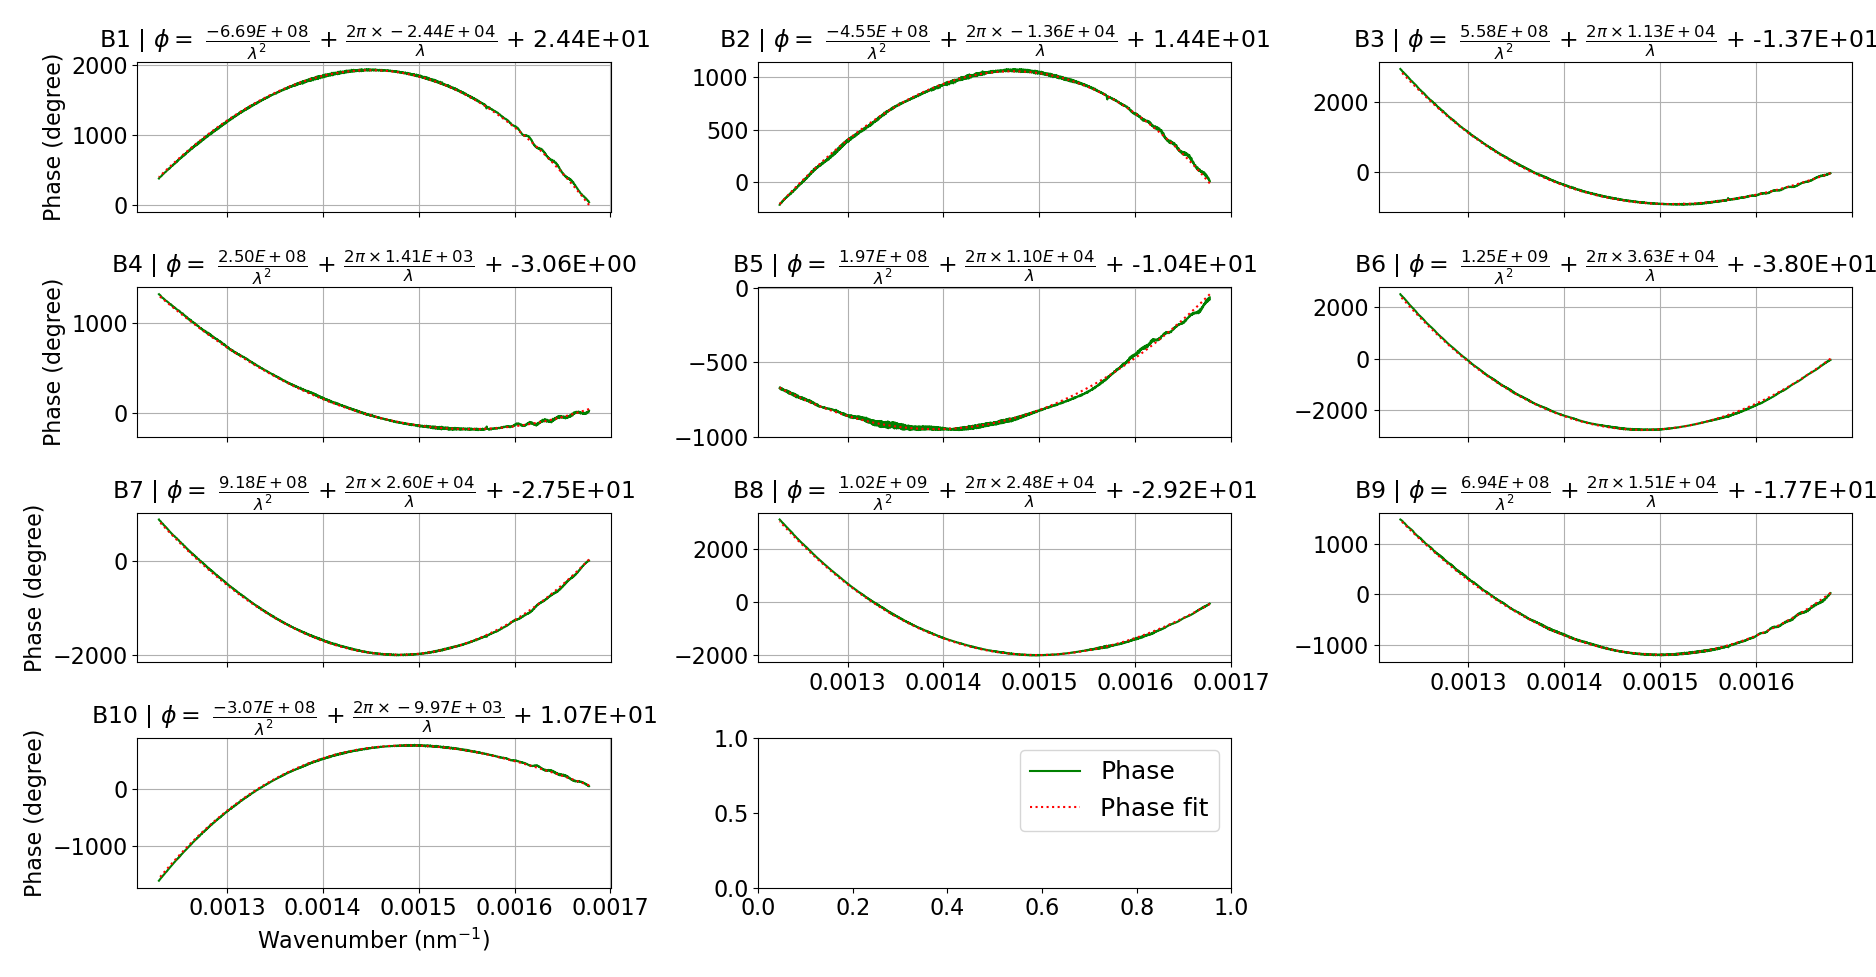
\includegraphics[width=\figwidth]{Figure_Chap3/20221010_Bin01_PhaseFit_Pola1_BaseSubplot_LaTex.png}
    \caption[Phases mesurées et ajustées en fonction du nombre d'onde sur la puce $Y$.]{Phases mesurées déroulées (en vert) et leur ajustement (en rouge) en fonction du nombre d'onde pour la puce $Y$. Les numéros des bases sont indiqués dans le titre de chaque graphique par la dénomination \textit{B\#} et suivis par les termes du polynôme de second degré ajusté aux phases.}
    \label{fig:FitPhaseVis}
\end{figure}

Les phases différentielles résultantes de la soustraction entre les fonctions ajustées et les phases mesurées sont tracées sur la figure~\ref{fig:PhaseDiffEx} et seront analysées plus loin dans la section~\ref{sec:PhaseDiffAnalyse}.

\begin{figure}[ht!]
    \centering
    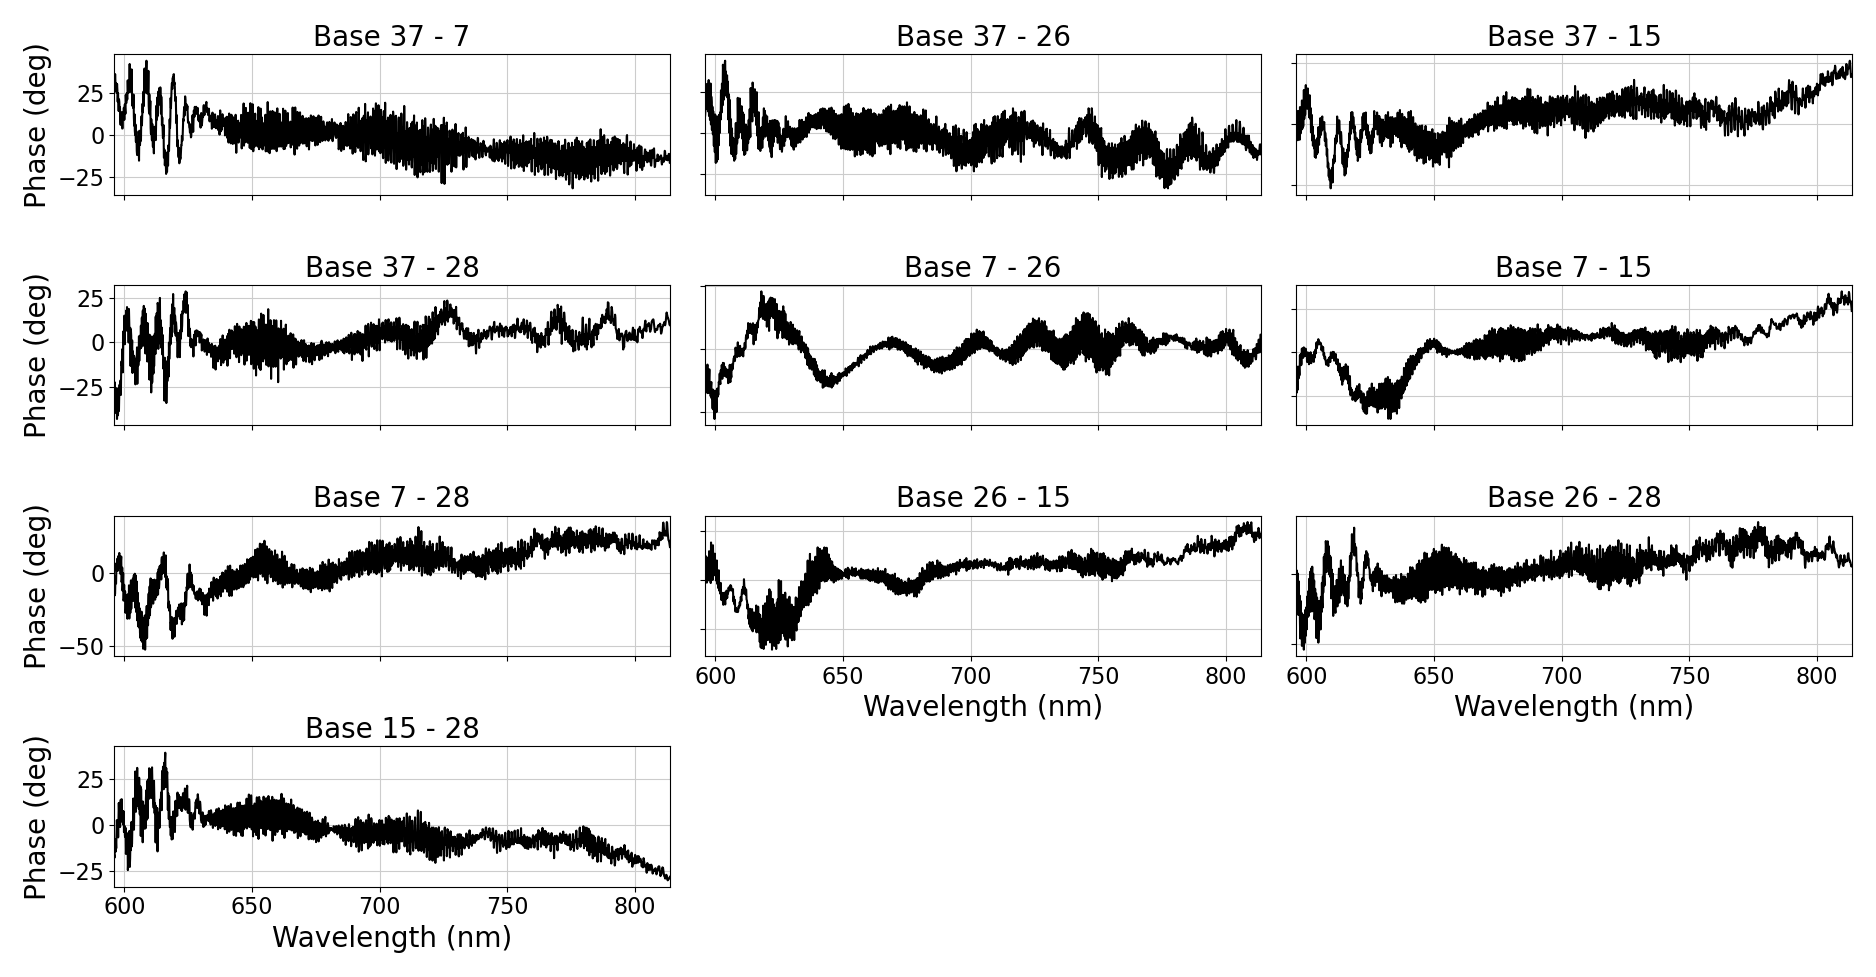
\includegraphics[width=\figwidth]{Figure_Chap4/20221010_SpeDiffPhase_BaseSubplot_Pola1_LaTex.png}
    \caption[Phases différentielles mesurées sur la source interne du banc de test.]{Phases différentielles mesurées sur la source interne du banc de test (non résolue), pour les dix bases de FIRSTv2, avec la puce $Y$. Les mesures sont présentées en fonction de la longueur d'onde entre $620 \,$nm et $660 \,$nm.}
    \label{fig:PhaseDiffEx}
\end{figure}


%%%%%%%%%%%%%%%%
\subsection{Les intérêts de la phase différentielle}

Comme nous l'avons vu, la phase différentielle est une observable auto-étalonnée des pistons atmosphériques et des biais instrumentaux. Du fait qu'elle s'obtienne par la soustraction du signal de la cible observée sur quelques canaux spectraux de travail par le signal du continuum sur le reste de la bande spectrale, il se trouve qu'elle est très bien adaptée au cas scientifique qui m'intéresse dans le cadre de ma thèse. En effet, comme je l'ai présenté dans la section~\ref{sec:Protoplanetes}, les protoplanètes en accrétion de matière émettent une forte raie d'émission \ha. Le signal de phase mesuré par \ac{FIRSTv2} sur un tel système présenterait alors un fort pic sur quelques canaux spectraux (canaux de travail), ce qui se prête bien au calcul de la phase différentielle.

De plus, il n'est pas nécessaire d'observer une cible non-résolue (de référence) pour étalonner les phases différentielles, contrairement aux clôtures de phase. C'est un avantage considérable car cela nécessite moins de temps d'observations sur télescope (rare et précieux).

Enfin, la phase différentielle est une observable au premier ordre et à la différence des clôtures de phase qui sont au troisième ordre. Pour N sous-pupilles combinées, on obtient $N(N-1)/2$ phases différentielles indépendantes et $(N-1)(N-2)/2$ clôtures de phase indépendantes. Ainsi, pour $5$ sous-pupilles on obtient $10$ phases différentielles indépendantes et $6$ clôtures de phase indépendantes \citep{millour2006}.


%%%%%%%%%%%%%%%%%%%%%%%%%%%%%%%%
\section{La stabilité des mesures sur le banc FIRSTv2}
\label{sec:CPStabilityMeudon}

Pour caractériser la stabilité des mesures de phases sur le banc de test de \ac{FIRSTv2}, j'acquiers des données sur la source interne non résolue. Ainsi, on s'attend à ce que le module des visibilités complexes estimées sur une telle source soit égale à $|V_{nn'}| = 1$ et sa phase à $\varphi_{nn'} = 0$. Par conséquent, l'équation~\ref{eq:mu} du terme de cohérence complexe de la base formée par les sous-pupilles $n$ et $n'$ devient $\mu_{nn'} = A_n A_{n'} e^{i(\Delta\Phi_{nn'})}$. La mesure de la phase de la cohérence complexe sur la source interne revient donc à mesurer le piston différentiel des perturbations sur le banc $\Delta\Phi_{nn'} = 2 \pi \sigma \delta_{nn'} [2 \pi]$. Pour ce faire, une fonction polynomiale d'ordre $2$ est ajustée à chaque mesure de phase déroulée selon la méthode présentée dans la section~\ref{sec:PhaseDiffFIRSTv2}, ce qui permet d'extraire le terme d'\ac{OPD} $\delta_{nn'}$, qui est le coefficient du terme polynomial d'ordre $1$.

Ainsi, la figure~\ref{fig:OPDfitVStime} est un graphique qui trace en fonction du temps, l'\ac{OPD} des bases $37-7$, $37-15$ et $7-15$ (en haut) et la clôture de phase \citep{weigelt1977, lohmann1983} associée est tracée en rouge (en bas). Les courbes sont tracées pour $1\,980$ images de temps d'exposition égal à $100 \,$ms. La moyenne de chaque courbe est tracée en trait discontinu noir et celle de la clôture de phase vaut $\upmu = 90 \,$nm avec comme écart-type $\sigma = 50 \,$nm. L'écart-type des \ac{OPD}s sont estimées à $90 \,$nm, $130 \,$nm et $80 \,$nm, respectivement. Cela montre que le calcul de la clôture de phase corrige les perturbations présentes sur le banc.

\begin{figure}[ht!]
    \centering
    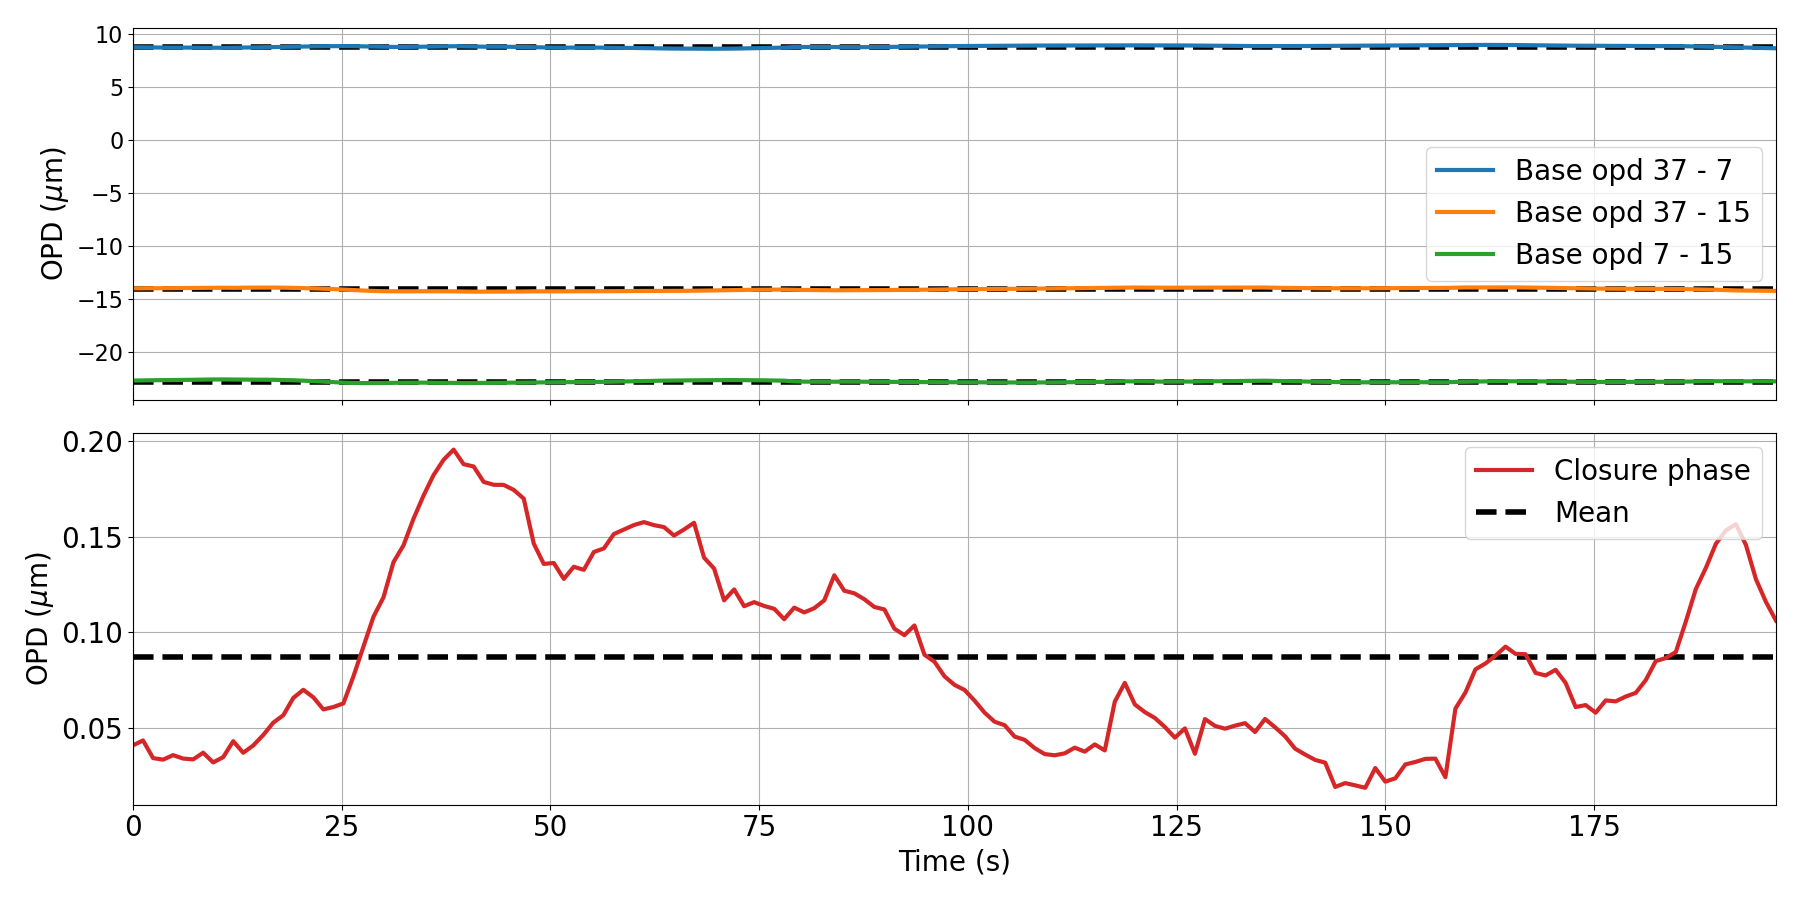
\includegraphics[width=\figwidth]{Figure_Chap3/20221010_FullOnData_OPDFitCPvsTime_CP2_Pola1_Base_LaTex.png}
    \caption[Graphique de l'OPD de trois bases et de la clôture de phase en fonction du temps, mesurée sur FIRSTv2 avec la puce $Y$.]{Graphique de l'OPD des bases $37-7$, $37-15$ et $7-15$ (en haut), en fonction du temps, mesurée sur FIRSTv2 avec la puce $Y$. La clôture de phase formée par ces trois bases est tracée en rouge (en bas) et les moyennes des quatre courbes sont tracées en trait noir discontinue. La moyenne de la clôture de phase est égale à $90 \,$nm et l'écart-type est de $50 \,$nm. Les courbes sont tracées pour $1\,980$ images de temps d'exposition égal à $100 \,$ms.}
    \label{fig:OPDfitVStime}
\end{figure}

Sous l'hypothèse que les variations temporelles des perturbations instrumentales se moyennent à zéro, le terme d'\ac{OPD} $\delta_{nn'}$ mesuré est la différence de longueur de chemin optique entre les faisceaux. La figure~\ref{fig:FiberPiston} montre les longueurs relatives des cinq bras de \ac{FIRSTv2}, induites par résolution du système d'équation linéaire reliant les \ac{OPD}s précédemment présentées aux longueurs de chemin relatives des bras. Chaque faisceau est identifié par le numéro du segment du \ac{MEMS} qu'il illumine (axe des abscisses). Les segments utilisés sont ceux présentés dans la section~\ref{sec:BaseConfig}. Il faut noter que ce sont les valeurs de longueurs relatives des faisceaux au moment de la mesure et celles-ci peuvent être minimisées en changeant les positions des \ac{ODL}s, rapprochant les interférogrammes de la frange centrale d'\ac{OPD} nulle.

\begin{figure}[ht!]
    \centering
    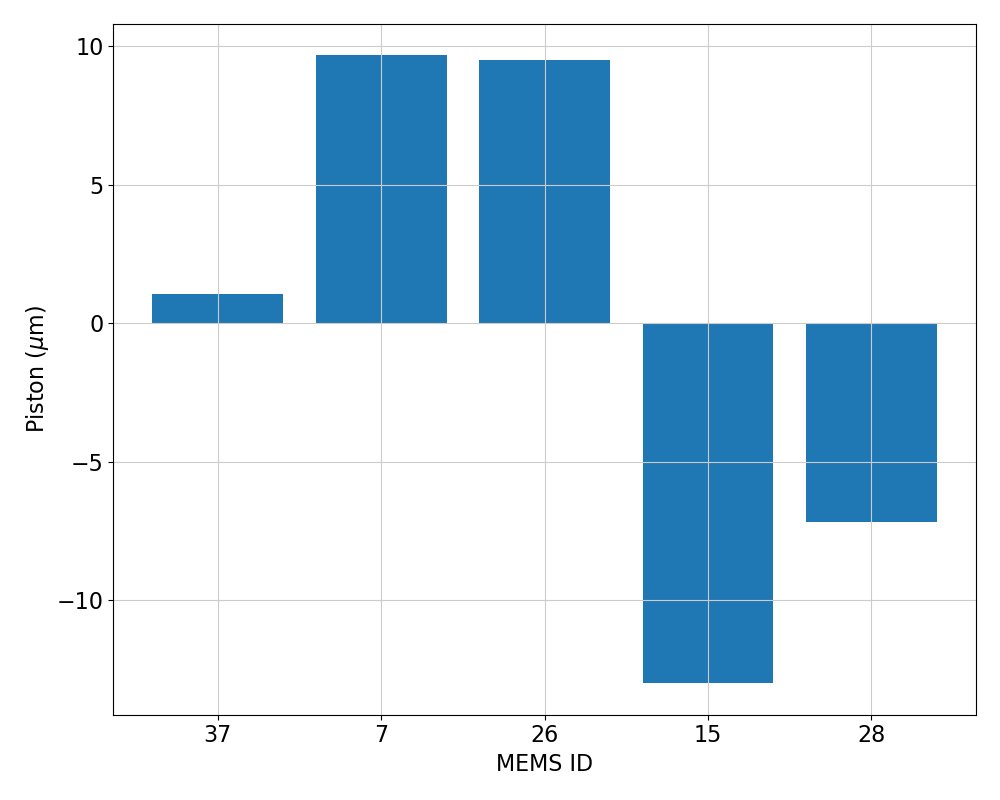
\includegraphics[width=\figwidth]{Figure_Chap3/20221010_FullOnData_FiberPiston_Pola1_LaTex.png}
    \caption[Longueurs relatives des $5$ bras de l'interféromètre de FIRSTv2, mesurées avec la puce $Y$.]{Longueurs relatives des $5$ bras de l'interféromètre de FIRSTv2, mesurées avec la puce $Y$. Chaque faisceau est identifié par le numéro du segment du MEMS qu'il illumine (axe des abscisses).}
    \label{fig:FiberPiston}
\end{figure}


%%%%%%%%%%%%%%%%%%%%%%%%%%%%%%%%
\section{Conclusion}

Dans ce chapitre j'ai présenté le processus du traitement des données de \ac{FIRSTv2} que j'ai développé pendant ma thèse. Celui-ci se base sur la méthode de calcul de la \ac{P2VM} qui est implémentée pour \ac{FIRSTv1} et précédemment pour \ac{AMBER}.

On a vu les différents étalonnages de l'instrument qui sont primordiaux dans le processus du traitement de données. Notamment l'étalonnage spectral sur toutes les sorties imagées sur le détecteur permettant l'identification des canal spectraux sur les pixels de la caméra. Mais encore, j'ai présenté tout le processus d'étalonnage de la \ac{P2VM} consistant à estimer la phase des interférogrammes pour chaque pas d'une séquence de modulation des franges connue et appliquée sur les segments du \ac{MEMS}.

Enfin, j'ai présenté la phase différentielle qui est une observable permettant de s'affranchir des perturbations instrumentales de bas ordres et que j'ai implémenté dans le programme de traitement de données pendant ma thèse. La phase différentielle est adaptée à la mesure interférométrique sur des sources lumineuses telles que les systèmes protoplanétaires dont le compagnon présente un faible contraste dans une raie d'émission. Elle sera exploitée dans le chapitre suivant pour l'analyse des données acquises sur un système protoplanétaire simulé sur le banc de test.
